\documentclass[twoside]{book}

% Packages required by doxygen
\usepackage{fixltx2e}
\usepackage{calc}
\usepackage{doxygen}
\usepackage[export]{adjustbox} % also loads graphicx
\usepackage{graphicx}
\usepackage[utf8]{inputenc}
\usepackage{makeidx}
\usepackage{multicol}
\usepackage{multirow}
\PassOptionsToPackage{warn}{textcomp}
\usepackage{textcomp}
\usepackage[nointegrals]{wasysym}
\usepackage[table]{xcolor}

% Font selection
\usepackage[T1]{fontenc}
\usepackage[scaled=.90]{helvet}
\usepackage{courier}
\usepackage{amssymb}
\usepackage{sectsty}
\renewcommand{\familydefault}{\sfdefault}
\allsectionsfont{%
  \fontseries{bc}\selectfont%
  \color{darkgray}%
}
\renewcommand{\DoxyLabelFont}{%
  \fontseries{bc}\selectfont%
  \color{darkgray}%
}
\newcommand{\+}{\discretionary{\mbox{\scriptsize$\hookleftarrow$}}{}{}}

% Page & text layout
\usepackage{geometry}
\geometry{%
  a4paper,%
  top=2.5cm,%
  bottom=2.5cm,%
  left=2.5cm,%
  right=2.5cm%
}
\tolerance=750
\hfuzz=15pt
\hbadness=750
\setlength{\emergencystretch}{15pt}
\setlength{\parindent}{0cm}
\setlength{\parskip}{3ex plus 2ex minus 2ex}
\makeatletter
\renewcommand{\paragraph}{%
  \@startsection{paragraph}{4}{0ex}{-1.0ex}{1.0ex}{%
    \normalfont\normalsize\bfseries\SS@parafont%
  }%
}
\renewcommand{\subparagraph}{%
  \@startsection{subparagraph}{5}{0ex}{-1.0ex}{1.0ex}{%
    \normalfont\normalsize\bfseries\SS@subparafont%
  }%
}
\makeatother

% Headers & footers
\usepackage{fancyhdr}
\pagestyle{fancyplain}
\fancyhead[LE]{\fancyplain{}{\bfseries\thepage}}
\fancyhead[CE]{\fancyplain{}{}}
\fancyhead[RE]{\fancyplain{}{\bfseries\leftmark}}
\fancyhead[LO]{\fancyplain{}{\bfseries\rightmark}}
\fancyhead[CO]{\fancyplain{}{}}
\fancyhead[RO]{\fancyplain{}{\bfseries\thepage}}
\fancyfoot[LE]{\fancyplain{}{}}
\fancyfoot[CE]{\fancyplain{}{}}
\fancyfoot[RE]{\fancyplain{}{\bfseries\scriptsize Generated by Doxygen }}
\fancyfoot[LO]{\fancyplain{}{\bfseries\scriptsize Generated by Doxygen }}
\fancyfoot[CO]{\fancyplain{}{}}
\fancyfoot[RO]{\fancyplain{}{}}
\renewcommand{\footrulewidth}{0.4pt}
\renewcommand{\chaptermark}[1]{%
  \markboth{#1}{}%
}
\renewcommand{\sectionmark}[1]{%
  \markright{\thesection\ #1}%
}

% Indices & bibliography
\usepackage{natbib}
\usepackage[titles]{tocloft}
\setcounter{tocdepth}{3}
\setcounter{secnumdepth}{5}
\makeindex

% Hyperlinks (required, but should be loaded last)
\usepackage{ifpdf}
\ifpdf
  \usepackage[pdftex,pagebackref=true]{hyperref}
\else
  \usepackage[ps2pdf,pagebackref=true]{hyperref}
\fi
\hypersetup{%
  colorlinks=true,%
  linkcolor=blue,%
  citecolor=blue,%
  unicode%
}

% Custom commands
\newcommand{\clearemptydoublepage}{%
  \newpage{\pagestyle{empty}\cleardoublepage}%
}

\usepackage{caption}
\captionsetup{labelsep=space,justification=centering,font={bf},singlelinecheck=off,skip=4pt,position=top}

%===== C O N T E N T S =====

\begin{document}

% Titlepage & ToC
\hypersetup{pageanchor=false,
             bookmarksnumbered=true,
             pdfencoding=unicode
            }
\pagenumbering{alph}
\begin{titlepage}
\vspace*{7cm}
\begin{center}%
{\Large Stock\+Market—\+A\+E\+DA \\[1ex]\large 2 }\\
\vspace*{1cm}
{\large Generated by Doxygen 1.8.12}\\
\end{center}
\end{titlepage}
\clearemptydoublepage
\pagenumbering{roman}
\tableofcontents
\clearemptydoublepage
\pagenumbering{arabic}
\hypersetup{pageanchor=true}

%--- Begin generated contents ---
\chapter{Hierarchical Index}
\section{Class Hierarchy}
This inheritance list is sorted roughly, but not completely, alphabetically\+:\begin{DoxyCompactList}
\item \contentsline{section}{Client}{\pageref{class_client}}{}
\item \contentsline{section}{client\+Ptr\+Hash}{\pageref{structclient_ptr_hash}}{}
\item \contentsline{section}{Date}{\pageref{class_date}}{}
\item \contentsline{section}{Client\+:\+:Invalid\+N\+IF}{\pageref{class_client_1_1_invalid_n_i_f}}{}
\item \contentsline{section}{Manager\+:\+:Invalid\+Password}{\pageref{class_manager_1_1_invalid_password}}{}
\item \contentsline{section}{Order\+:\+:Invalid\+Value}{\pageref{class_order_1_1_invalid_value}}{}
\item \contentsline{section}{Manager}{\pageref{class_manager}}{}
\item \contentsline{section}{Market}{\pageref{class_market}}{}
\item \contentsline{section}{News}{\pageref{class_news}}{}
\item \contentsline{section}{Order}{\pageref{class_order}}{}
\begin{DoxyCompactList}
\item \contentsline{section}{Buy\+Order}{\pageref{class_buy_order}}{}
\item \contentsline{section}{Sell\+Order}{\pageref{class_sell_order}}{}
\end{DoxyCompactList}
\item \contentsline{section}{Transaction}{\pageref{class_transaction}}{}
\end{DoxyCompactList}

\chapter{Class Index}
\section{Class List}
Here are the classes, structs, unions and interfaces with brief descriptions\+:\begin{DoxyCompactList}
\item\contentsline{section}{\hyperlink{class_buy_order}{Buy\+Order} }{\pageref{class_buy_order}}{}
\item\contentsline{section}{\hyperlink{class_client}{Client} }{\pageref{class_client}}{}
\item\contentsline{section}{\hyperlink{structclient_ptr_hash}{client\+Ptr\+Hash} }{\pageref{structclient_ptr_hash}}{}
\item\contentsline{section}{\hyperlink{class_date}{Date} }{\pageref{class_date}}{}
\item\contentsline{section}{\hyperlink{class_client_1_1_invalid_n_i_f}{Client\+::\+Invalid\+N\+IF} }{\pageref{class_client_1_1_invalid_n_i_f}}{}
\item\contentsline{section}{\hyperlink{class_manager_1_1_invalid_password}{Manager\+::\+Invalid\+Password} }{\pageref{class_manager_1_1_invalid_password}}{}
\item\contentsline{section}{\hyperlink{class_order_1_1_invalid_value}{Order\+::\+Invalid\+Value} }{\pageref{class_order_1_1_invalid_value}}{}
\item\contentsline{section}{\hyperlink{class_manager}{Manager} }{\pageref{class_manager}}{}
\item\contentsline{section}{\hyperlink{class_market}{Market} }{\pageref{class_market}}{}
\item\contentsline{section}{\hyperlink{class_news}{News} }{\pageref{class_news}}{}
\item\contentsline{section}{\hyperlink{class_order}{Order} }{\pageref{class_order}}{}
\item\contentsline{section}{\hyperlink{class_sell_order}{Sell\+Order} }{\pageref{class_sell_order}}{}
\item\contentsline{section}{\hyperlink{class_transaction}{Transaction} }{\pageref{class_transaction}}{}
\end{DoxyCompactList}

\chapter{Class Documentation}
\hypertarget{class_buy_order}{}\section{Buy\+Order Class Reference}
\label{class_buy_order}\index{Buy\+Order@{Buy\+Order}}


{\ttfamily \#include $<$Order.\+h$>$}

Inheritance diagram for Buy\+Order\+:\begin{figure}[H]
\begin{center}
\leavevmode
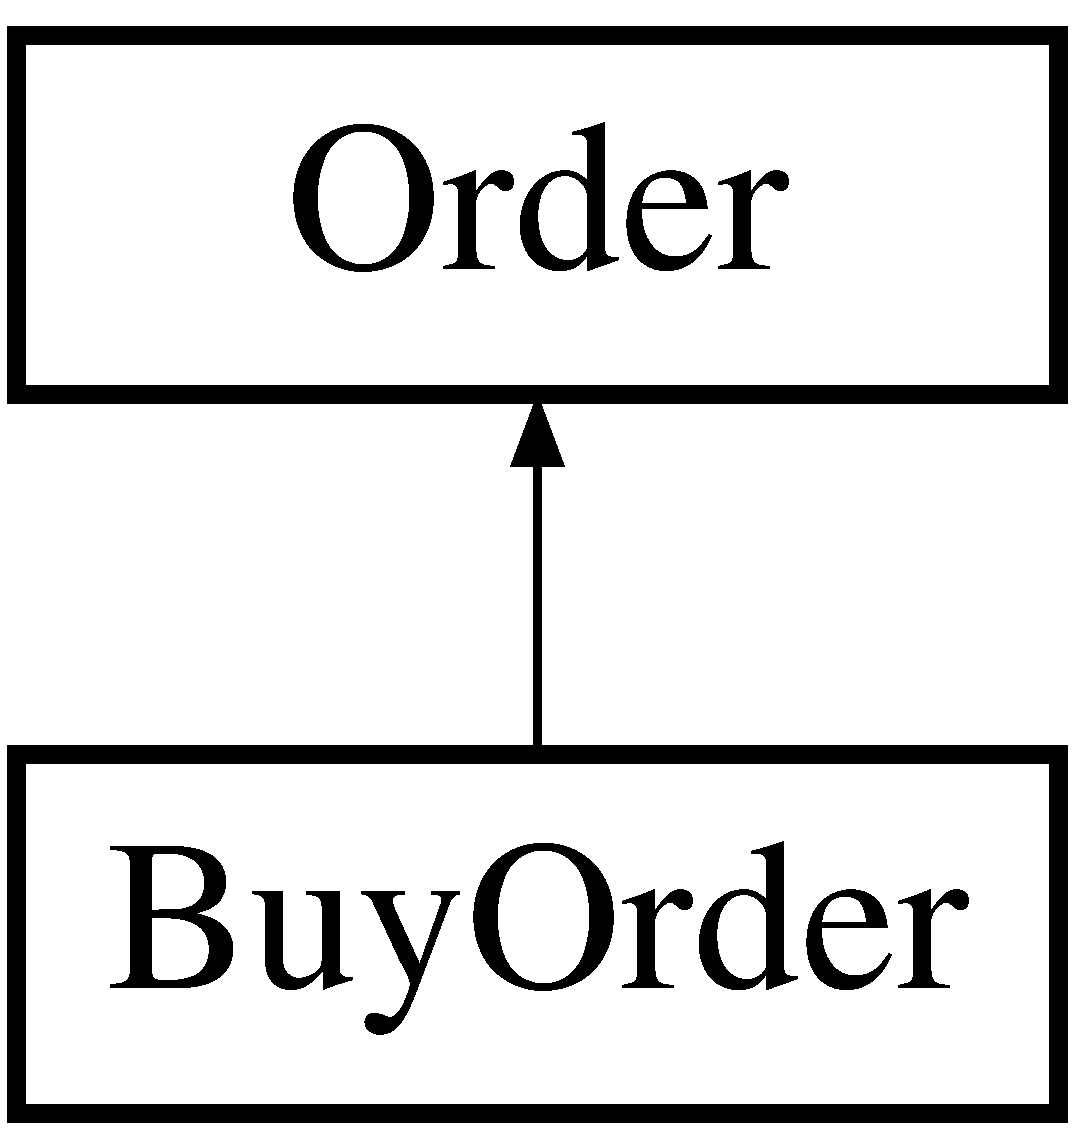
\includegraphics[height=2.000000cm]{class_buy_order}
\end{center}
\end{figure}
\subsection*{Public Member Functions}
\begin{DoxyCompactItemize}
\item 
\hyperlink{class_buy_order_acbf093767d9d108b9448f2eefb5f58cd}{Buy\+Order} (ifstream \&in)
\begin{DoxyCompactList}\small\item\em /// \end{DoxyCompactList}\item 
\hyperlink{class_buy_order_a1fcd1c4a28acdf04bfdf99c5b16b4e7d}{Buy\+Order} (string \hyperlink{class_order_aafb6dfab2a1c253eefd78840b27dcd2e}{stock}, double val, unsigned \hyperlink{class_order_ab02e2baeb8c57217a20c9124df3ba11d}{quantity}, nif\+\_\+t buyer\+N\+IF)
\item 
nif\+\_\+t \hyperlink{class_buy_order_ab79597b9bf0656216b2283bfa3a650e0}{get\+Client\+N\+IF} () const
\item 
\hyperlink{class_transaction}{Transaction} $\ast$ \hyperlink{class_buy_order_a45641eed13ea191fff675745a618b9f5}{operator()} (\hyperlink{class_order}{Order} $\ast$o)
\item 
void \hyperlink{class_buy_order_aa4f087d0dbc1f6e8937c0b3679fc2f7b}{save\+Changes} (ofstream \&out) const
\end{DoxyCompactItemize}
\subsection*{Additional Inherited Members}


\subsection{Detailed Description}
Class used to represent a buy order. Derives from \hyperlink{class_order}{Order}. 

\subsection{Constructor \& Destructor Documentation}
\hypertarget{class_buy_order_acbf093767d9d108b9448f2eefb5f58cd}{}\label{class_buy_order_acbf093767d9d108b9448f2eefb5f58cd} 
\index{Buy\+Order@{Buy\+Order}!Buy\+Order@{Buy\+Order}}
\index{Buy\+Order@{Buy\+Order}!Buy\+Order@{Buy\+Order}}
\subsubsection{\texorpdfstring{Buy\+Order()}{BuyOrder()}\hspace{0.1cm}{\footnotesize\ttfamily [1/2]}}
{\footnotesize\ttfamily Buy\+Order\+::\+Buy\+Order (\begin{DoxyParamCaption}\item[{ifstream \&}]{in }\end{DoxyParamCaption})}



/// 

A constructor. The construtor creates a \hyperlink{class_buy_order}{Buy\+Order} object, reading the data from the input stream passed as argument. 
\begin{DoxyParams}{Parameters}
{\em in} & The input stream to read from in order to build the \hyperlink{class_buy_order}{Buy\+Order} object. \\
\hline
\end{DoxyParams}
\hypertarget{class_buy_order_a1fcd1c4a28acdf04bfdf99c5b16b4e7d}{}\label{class_buy_order_a1fcd1c4a28acdf04bfdf99c5b16b4e7d} 
\index{Buy\+Order@{Buy\+Order}!Buy\+Order@{Buy\+Order}}
\index{Buy\+Order@{Buy\+Order}!Buy\+Order@{Buy\+Order}}
\subsubsection{\texorpdfstring{Buy\+Order()}{BuyOrder()}\hspace{0.1cm}{\footnotesize\ttfamily [2/2]}}
{\footnotesize\ttfamily Buy\+Order\+::\+Buy\+Order (\begin{DoxyParamCaption}\item[{string}]{stock,  }\item[{double}]{val,  }\item[{unsigned}]{quantity,  }\item[{nif\+\_\+t}]{buyer\+N\+IF }\end{DoxyParamCaption})}

A constructor. The construtor creates a \hyperlink{class_buy_order}{Buy\+Order} object using the data passed as arguments. 
\begin{DoxyParams}{Parameters}
{\em stock} & A string with the stock name. \\
\hline
{\em val} & A double with the value per stock. \\
\hline
{\em quantity} & An unsigned with the stock quantity. \\
\hline
{\em buyer\+N\+IF} & The buyer\textquotesingle{}s N\+IF. \\
\hline
\end{DoxyParams}


\subsection{Member Function Documentation}
\hypertarget{class_buy_order_ab79597b9bf0656216b2283bfa3a650e0}{}\label{class_buy_order_ab79597b9bf0656216b2283bfa3a650e0} 
\index{Buy\+Order@{Buy\+Order}!get\+Client\+N\+IF@{get\+Client\+N\+IF}}
\index{get\+Client\+N\+IF@{get\+Client\+N\+IF}!Buy\+Order@{Buy\+Order}}
\subsubsection{\texorpdfstring{get\+Client\+N\+I\+F()}{getClientNIF()}}
{\footnotesize\ttfamily nif\+\_\+t Buy\+Order\+::get\+Client\+N\+IF (\begin{DoxyParamCaption}{ }\end{DoxyParamCaption}) const\hspace{0.3cm}{\ttfamily [virtual]}}

A const member function that returns the N\+IF of the client associated with this \hyperlink{class_buy_order}{Buy\+Order}. \begin{DoxyReturn}{Returns}
The N\+IF of the Buyer associated with this \hyperlink{class_order}{Order}. 
\end{DoxyReturn}


Implements \hyperlink{class_order_a9831f386726f74ee20eea13a46282e13}{Order}.

\hypertarget{class_buy_order_a45641eed13ea191fff675745a618b9f5}{}\label{class_buy_order_a45641eed13ea191fff675745a618b9f5} 
\index{Buy\+Order@{Buy\+Order}!operator()@{operator()}}
\index{operator()@{operator()}!Buy\+Order@{Buy\+Order}}
\subsubsection{\texorpdfstring{operator()()}{operator()()}}
{\footnotesize\ttfamily \hyperlink{class_transaction}{Transaction} $\ast$ Buy\+Order\+::operator() (\begin{DoxyParamCaption}\item[{\hyperlink{class_order}{Order} $\ast$}]{o }\end{DoxyParamCaption})\hspace{0.3cm}{\ttfamily [virtual]}}

Overload of operator() for class \hyperlink{class_order}{Order}. 
\begin{DoxyParams}{Parameters}
{\em o} & Pointer of an object \hyperlink{class_order}{Order}. \\
\hline
\end{DoxyParams}
\begin{DoxyReturn}{Returns}
A transaction type object. 
\end{DoxyReturn}


Implements \hyperlink{class_order_a85d5de18c8664085619e3a5c74d47a25}{Order}.

\hypertarget{class_buy_order_aa4f087d0dbc1f6e8937c0b3679fc2f7b}{}\label{class_buy_order_aa4f087d0dbc1f6e8937c0b3679fc2f7b} 
\index{Buy\+Order@{Buy\+Order}!save\+Changes@{save\+Changes}}
\index{save\+Changes@{save\+Changes}!Buy\+Order@{Buy\+Order}}
\subsubsection{\texorpdfstring{save\+Changes()}{saveChanges()}}
{\footnotesize\ttfamily void Buy\+Order\+::save\+Changes (\begin{DoxyParamCaption}\item[{ofstream \&}]{out }\end{DoxyParamCaption}) const\hspace{0.3cm}{\ttfamily [virtual]}}

A const memeber function to save changes in an output stream. 
\begin{DoxyParams}{Parameters}
{\em out} & The outstream file to write to. \\
\hline
\end{DoxyParams}


Reimplemented from \hyperlink{class_order_a83989bde0a9b40cbeb0e87c965f6096e}{Order}.



The documentation for this class was generated from the following files\+:\begin{DoxyCompactItemize}
\item 
Order.\+h\item 
Order.\+cpp\end{DoxyCompactItemize}

\hypertarget{class_client}{}\section{Client Class Reference}
\label{class_client}\index{Client@{Client}}


{\ttfamily \#include $<$Client.\+h$>$}

\subsection*{Classes}
\begin{DoxyCompactItemize}
\item 
class \hyperlink{class_client_1_1_invalid_n_i_f}{Invalid\+N\+IF}
\end{DoxyCompactItemize}
\subsection*{Public Member Functions}
\begin{DoxyCompactItemize}
\item 
\hyperlink{class_client_ac13ad1e98c47db57ce0823dc735261cd}{Client} ()=default
\item 
\hyperlink{class_client_a978037b72169d091a54867507ecd38ed}{Client} (ifstream \&in)
\item 
\hyperlink{class_client_a6e10627d296d1fb74f092935784356e3}{Client} (string name, nif\+\_\+t nif, string address, string contact)
\item 
string \hyperlink{class_client_a5c473ba52d7678744edec9e51052c947}{get\+Name} () const
\item 
string \hyperlink{class_client_ac78e5756e7151f9bdfc2662dd4cab207}{get\+Contact} () const
\item 
string \hyperlink{class_client_afdf2c15b5ef6f4069786077717702a3f}{get\+Address} () const
\item 
nif\+\_\+t \hyperlink{class_client_a2f9bc46f381dcbd0f35929f54dabad59}{get\+N\+IF} () const
\item 
bool \hyperlink{class_client_ac55e135fde79306fd9892edf9d4a3d3c}{set\+Address} (string address)
\item 
bool \hyperlink{class_client_a8ea7024b571a3145a3de24fc526790ae}{set\+Contact} (string contact)
\item 
void \hyperlink{class_client_a3bd7a77458497b3b863b7c7515d76e68}{save\+Changes} (ofstream \&out) const
\end{DoxyCompactItemize}


\subsection{Detailed Description}
A class used to represent a client. Each client object has a name and a nif (from the portuguese \char`\"{}\+Numero de Identifica��o Fiscal\char`\"{}). 

\subsection{Constructor \& Destructor Documentation}
\hypertarget{class_client_ac13ad1e98c47db57ce0823dc735261cd}{}\label{class_client_ac13ad1e98c47db57ce0823dc735261cd} 
\index{Client@{Client}!Client@{Client}}
\index{Client@{Client}!Client@{Client}}
\subsubsection{\texorpdfstring{Client()}{Client()}\hspace{0.1cm}{\footnotesize\ttfamily [1/3]}}
{\footnotesize\ttfamily Client\+::\+Client (\begin{DoxyParamCaption}{ }\end{DoxyParamCaption})\hspace{0.3cm}{\ttfamily [default]}}

Explicit default constructor. \hypertarget{class_client_a978037b72169d091a54867507ecd38ed}{}\label{class_client_a978037b72169d091a54867507ecd38ed} 
\index{Client@{Client}!Client@{Client}}
\index{Client@{Client}!Client@{Client}}
\subsubsection{\texorpdfstring{Client()}{Client()}\hspace{0.1cm}{\footnotesize\ttfamily [2/3]}}
{\footnotesize\ttfamily Client\+::\+Client (\begin{DoxyParamCaption}\item[{ifstream \&}]{in }\end{DoxyParamCaption})}

Constructor from file. The construtor creates a \hyperlink{class_client}{Client} object, reading the data from the input stream passed as argument. 
\begin{DoxyParams}{Parameters}
{\em in} & The input stream to read from in order to build the client object. \\
\hline
\end{DoxyParams}
\hypertarget{class_client_a6e10627d296d1fb74f092935784356e3}{}\label{class_client_a6e10627d296d1fb74f092935784356e3} 
\index{Client@{Client}!Client@{Client}}
\index{Client@{Client}!Client@{Client}}
\subsubsection{\texorpdfstring{Client()}{Client()}\hspace{0.1cm}{\footnotesize\ttfamily [3/3]}}
{\footnotesize\ttfamily Client\+::\+Client (\begin{DoxyParamCaption}\item[{string}]{name,  }\item[{nif\+\_\+t}]{nif,  }\item[{string}]{address,  }\item[{string}]{contact }\end{DoxyParamCaption})}

A constructor. The construtor creates a client object with the data passed as arguments. 
\begin{DoxyParams}{Parameters}
{\em name} & The client\textquotesingle{}s name. \\
\hline
{\em nif} & The client\textquotesingle{}s N\+IF. \\
\hline
{\em address} & The client\textquotesingle{}s address. \\
\hline
{\em contact} & The client\textquotesingle{}s contact information. \\
\hline
\end{DoxyParams}


\subsection{Member Function Documentation}
\hypertarget{class_client_afdf2c15b5ef6f4069786077717702a3f}{}\label{class_client_afdf2c15b5ef6f4069786077717702a3f} 
\index{Client@{Client}!get\+Address@{get\+Address}}
\index{get\+Address@{get\+Address}!Client@{Client}}
\subsubsection{\texorpdfstring{get\+Address()}{getAddress()}}
{\footnotesize\ttfamily string Client\+::get\+Address (\begin{DoxyParamCaption}{ }\end{DoxyParamCaption}) const}

A const member function with no arguments to get the client\textquotesingle{}s address. \begin{DoxyReturn}{Returns}
A string, the client\textquotesingle{}s current address information. 
\end{DoxyReturn}
\hypertarget{class_client_ac78e5756e7151f9bdfc2662dd4cab207}{}\label{class_client_ac78e5756e7151f9bdfc2662dd4cab207} 
\index{Client@{Client}!get\+Contact@{get\+Contact}}
\index{get\+Contact@{get\+Contact}!Client@{Client}}
\subsubsection{\texorpdfstring{get\+Contact()}{getContact()}}
{\footnotesize\ttfamily string Client\+::get\+Contact (\begin{DoxyParamCaption}{ }\end{DoxyParamCaption}) const}

A const member function with no arguments to get the client\textquotesingle{}s contact information. \begin{DoxyReturn}{Returns}
A string, the client\textquotesingle{}s contact information. 
\end{DoxyReturn}
\hypertarget{class_client_a5c473ba52d7678744edec9e51052c947}{}\label{class_client_a5c473ba52d7678744edec9e51052c947} 
\index{Client@{Client}!get\+Name@{get\+Name}}
\index{get\+Name@{get\+Name}!Client@{Client}}
\subsubsection{\texorpdfstring{get\+Name()}{getName()}}
{\footnotesize\ttfamily string Client\+::get\+Name (\begin{DoxyParamCaption}{ }\end{DoxyParamCaption}) const}

A const member function with no arguments to get the client\textquotesingle{}s name. \begin{DoxyReturn}{Returns}
A string, the client\textquotesingle{}s name. 
\end{DoxyReturn}
\hypertarget{class_client_a2f9bc46f381dcbd0f35929f54dabad59}{}\label{class_client_a2f9bc46f381dcbd0f35929f54dabad59} 
\index{Client@{Client}!get\+N\+IF@{get\+N\+IF}}
\index{get\+N\+IF@{get\+N\+IF}!Client@{Client}}
\subsubsection{\texorpdfstring{get\+N\+I\+F()}{getNIF()}}
{\footnotesize\ttfamily nif\+\_\+t Client\+::get\+N\+IF (\begin{DoxyParamCaption}{ }\end{DoxyParamCaption}) const}

A const member function with no arguments to get the client\textquotesingle{}s N\+IF. \begin{DoxyReturn}{Returns}
A nif\+\_\+t, the client\textquotesingle{}s N\+IF. 
\end{DoxyReturn}
\hypertarget{class_client_a3bd7a77458497b3b863b7c7515d76e68}{}\label{class_client_a3bd7a77458497b3b863b7c7515d76e68} 
\index{Client@{Client}!save\+Changes@{save\+Changes}}
\index{save\+Changes@{save\+Changes}!Client@{Client}}
\subsubsection{\texorpdfstring{save\+Changes()}{saveChanges()}}
{\footnotesize\ttfamily void Client\+::save\+Changes (\begin{DoxyParamCaption}\item[{ofstream \&}]{out }\end{DoxyParamCaption}) const}

A const member function that writes the client\textquotesingle{}s info to the output stream. Generally used to save the client\textquotesingle{}s attributes to a file. 
\begin{DoxyParams}{Parameters}
{\em out} & The output stream to write the client\textquotesingle{}s information. \\
\hline
\end{DoxyParams}
\hypertarget{class_client_ac55e135fde79306fd9892edf9d4a3d3c}{}\label{class_client_ac55e135fde79306fd9892edf9d4a3d3c} 
\index{Client@{Client}!set\+Address@{set\+Address}}
\index{set\+Address@{set\+Address}!Client@{Client}}
\subsubsection{\texorpdfstring{set\+Address()}{setAddress()}}
{\footnotesize\ttfamily bool Client\+::set\+Address (\begin{DoxyParamCaption}\item[{string}]{address }\end{DoxyParamCaption})}

Changes the client\textquotesingle{}s address. 
\begin{DoxyParams}{Parameters}
{\em address} & The new address. \\
\hline
\end{DoxyParams}
\begin{DoxyReturn}{Returns}
A boolean, true if change was successful. 
\end{DoxyReturn}
\hypertarget{class_client_a8ea7024b571a3145a3de24fc526790ae}{}\label{class_client_a8ea7024b571a3145a3de24fc526790ae} 
\index{Client@{Client}!set\+Contact@{set\+Contact}}
\index{set\+Contact@{set\+Contact}!Client@{Client}}
\subsubsection{\texorpdfstring{set\+Contact()}{setContact()}}
{\footnotesize\ttfamily bool Client\+::set\+Contact (\begin{DoxyParamCaption}\item[{string}]{contact }\end{DoxyParamCaption})}

Changes the client\textquotesingle{}s contact information. 
\begin{DoxyParams}{Parameters}
{\em contact} & The new contact information. \\
\hline
\end{DoxyParams}
\begin{DoxyReturn}{Returns}
A boolean, true if change was successful. 
\end{DoxyReturn}


The documentation for this class was generated from the following files\+:\begin{DoxyCompactItemize}
\item 
Client.\+h\item 
Client.\+cpp\end{DoxyCompactItemize}

\hypertarget{structclient_ptr_hash}{}\section{client\+Ptr\+Hash Struct Reference}
\label{structclient_ptr_hash}\index{client\+Ptr\+Hash@{client\+Ptr\+Hash}}


{\ttfamily \#include $<$Client.\+h$>$}

\subsection*{Public Member Functions}
\begin{DoxyCompactItemize}
\item 
int \hyperlink{structclient_ptr_hash_ac49312a0983336d28135483f5e2c4f5c}{operator()} (const \hyperlink{class_client}{Client} $\ast$cli) const
\item 
bool \hyperlink{structclient_ptr_hash_adb7164b667757ee8091c7b7337b1be2b}{operator()} (const \hyperlink{class_client}{Client} $\ast$cli1, const \hyperlink{class_client}{Client} $\ast$cli2) const
\end{DoxyCompactItemize}


\subsection{Detailed Description}
A structure to encapsulate the Hash and Comparison functions of \hyperlink{class_client}{Client} Pointers. 

\subsection{Member Function Documentation}
\hypertarget{structclient_ptr_hash_ac49312a0983336d28135483f5e2c4f5c}{}\label{structclient_ptr_hash_ac49312a0983336d28135483f5e2c4f5c} 
\index{client\+Ptr\+Hash@{client\+Ptr\+Hash}!operator()@{operator()}}
\index{operator()@{operator()}!client\+Ptr\+Hash@{client\+Ptr\+Hash}}
\subsubsection{\texorpdfstring{operator()()}{operator()()}\hspace{0.1cm}{\footnotesize\ttfamily [1/2]}}
{\footnotesize\ttfamily int client\+Ptr\+Hash\+::operator() (\begin{DoxyParamCaption}\item[{const \hyperlink{class_client}{Client} $\ast$}]{cli }\end{DoxyParamCaption}) const\hspace{0.3cm}{\ttfamily [inline]}}

Hash Function for Client$\ast$ 
\begin{DoxyParams}{Parameters}
{\em cli} & Pointer to a \hyperlink{class_client}{Client} object. \\
\hline
\end{DoxyParams}
\begin{DoxyReturn}{Returns}
hash value. 
\end{DoxyReturn}
\hypertarget{structclient_ptr_hash_adb7164b667757ee8091c7b7337b1be2b}{}\label{structclient_ptr_hash_adb7164b667757ee8091c7b7337b1be2b} 
\index{client\+Ptr\+Hash@{client\+Ptr\+Hash}!operator()@{operator()}}
\index{operator()@{operator()}!client\+Ptr\+Hash@{client\+Ptr\+Hash}}
\subsubsection{\texorpdfstring{operator()()}{operator()()}\hspace{0.1cm}{\footnotesize\ttfamily [2/2]}}
{\footnotesize\ttfamily bool client\+Ptr\+Hash\+::operator() (\begin{DoxyParamCaption}\item[{const \hyperlink{class_client}{Client} $\ast$}]{cli1,  }\item[{const \hyperlink{class_client}{Client} $\ast$}]{cli2 }\end{DoxyParamCaption}) const\hspace{0.3cm}{\ttfamily [inline]}}

Comparison Function for Client$\ast$ 
\begin{DoxyParams}{Parameters}
{\em cli1} & Pointer to a \hyperlink{class_client}{Client} object. \\
\hline
{\em cli1} & Pointer to a \hyperlink{class_client}{Client} object. \\
\hline
\end{DoxyParams}
\begin{DoxyReturn}{Returns}
true if Clients pointed by cli1 and cli2 are the same, false otherwise. 
\end{DoxyReturn}


The documentation for this struct was generated from the following file\+:\begin{DoxyCompactItemize}
\item 
Client.\+h\end{DoxyCompactItemize}

\hypertarget{class_date}{}\section{Date Class Reference}
\label{class_date}\index{Date@{Date}}


{\ttfamily \#include $<$Date.\+h$>$}

\subsection*{Public Member Functions}
\begin{DoxyCompactItemize}
\item 
\hyperlink{class_date_a4e59ed4ba66eec61c27460c5d09fa1bd}{Date} ()
\item 
\hyperlink{class_date_aed0ec4ac9e00fb6130f8a642a61180b9}{Date} (string data)
\item 
\hyperlink{class_date_ab1ad19969fa570605a6b0cd32b0da822}{Date} (int day, int month, int year)
\item 
int \hyperlink{class_date_a86208bd42da6587c4b45ed93d688d483}{get\+\_\+day} () const
\item 
int \hyperlink{class_date_a89ae60bad421600e3ee901eb0df44975}{get\+\_\+month} () const
\item 
int \hyperlink{class_date_a9e77e9f49890449fea9aeb8114da95ff}{get\+\_\+year} () const
\end{DoxyCompactItemize}
\subsection*{Friends}
\begin{DoxyCompactItemize}
\item 
ostream \& \hyperlink{class_date_a5c29d00ecf33e6d232a410f1f3d6eb70}{operator$<$$<$} (ostream \&out, const \hyperlink{class_date}{Date} \&date)
\item 
istream \& \hyperlink{class_date_a5b292605462c1f43c993c0b2f5592cdc}{operator$>$$>$} (istream \&in, \hyperlink{class_date}{Date} \&date)
\item 
bool \hyperlink{class_date_a4f314b2216e8760eac284385a7eaae12}{operator$<$=} (const \hyperlink{class_date}{Date} \&d1, const \hyperlink{class_date}{Date} \&d2)
\item 
bool \hyperlink{class_date_a5a3f411cbd59e9ecb90b2f8e6aaea551}{operator$<$} (const \hyperlink{class_date}{Date} \&d1, const \hyperlink{class_date}{Date} \&d2)
\item 
bool \hyperlink{class_date_a18dc8aca1ca4d8cadc2b464db984135b}{operator==} (const \hyperlink{class_date}{Date} \&d1, const \hyperlink{class_date}{Date} \&d2)
\item 
bool \hyperlink{class_date_a15180616122b6ffa419f17a06aca3ec7}{operator!=} (const \hyperlink{class_date}{Date} \&d1, const \hyperlink{class_date}{Date} \&d2)
\item 
int \hyperlink{class_date_a90540af47999b64ed77651ece2ed3be5}{date\+Difference} (const \hyperlink{class_date}{Date} \&d1, const \hyperlink{class_date}{Date} \&d2)
\end{DoxyCompactItemize}


\subsection{Detailed Description}
A class used to represent a date. Each date object contains 3 integers, representing day, month and year. 

\subsection{Constructor \& Destructor Documentation}
\hypertarget{class_date_a4e59ed4ba66eec61c27460c5d09fa1bd}{}\label{class_date_a4e59ed4ba66eec61c27460c5d09fa1bd} 
\index{Date@{Date}!Date@{Date}}
\index{Date@{Date}!Date@{Date}}
\subsubsection{\texorpdfstring{Date()}{Date()}\hspace{0.1cm}{\footnotesize\ttfamily [1/3]}}
{\footnotesize\ttfamily Date\+::\+Date (\begin{DoxyParamCaption}{ }\end{DoxyParamCaption})}

A default constructor. The default construtor creates a date object with the current system date. \hypertarget{class_date_aed0ec4ac9e00fb6130f8a642a61180b9}{}\label{class_date_aed0ec4ac9e00fb6130f8a642a61180b9} 
\index{Date@{Date}!Date@{Date}}
\index{Date@{Date}!Date@{Date}}
\subsubsection{\texorpdfstring{Date()}{Date()}\hspace{0.1cm}{\footnotesize\ttfamily [2/3]}}
{\footnotesize\ttfamily Date\+::\+Date (\begin{DoxyParamCaption}\item[{string}]{data }\end{DoxyParamCaption})}

A constructor. The construtor creates a date object with the specified date string specified as argument. 
\begin{DoxyParams}{Parameters}
{\em data} & A string with the date in the D\+D/\+M\+M/\+YY format \\
\hline
\end{DoxyParams}
\hypertarget{class_date_ab1ad19969fa570605a6b0cd32b0da822}{}\label{class_date_ab1ad19969fa570605a6b0cd32b0da822} 
\index{Date@{Date}!Date@{Date}}
\index{Date@{Date}!Date@{Date}}
\subsubsection{\texorpdfstring{Date()}{Date()}\hspace{0.1cm}{\footnotesize\ttfamily [3/3]}}
{\footnotesize\ttfamily Date\+::\+Date (\begin{DoxyParamCaption}\item[{int}]{day,  }\item[{int}]{month,  }\item[{int}]{year }\end{DoxyParamCaption})}

A constructor. The construtor creates a date object with the specified day, month and year passed as arguments. 
\begin{DoxyParams}{Parameters}
{\em day} & A unsigned short representing the day \\
\hline
{\em month} & A unsigned short representing the month \\
\hline
{\em year} & A unsigned short representing the year \\
\hline
\end{DoxyParams}


\subsection{Member Function Documentation}
\hypertarget{class_date_a86208bd42da6587c4b45ed93d688d483}{}\label{class_date_a86208bd42da6587c4b45ed93d688d483} 
\index{Date@{Date}!get\+\_\+day@{get\+\_\+day}}
\index{get\+\_\+day@{get\+\_\+day}!Date@{Date}}
\subsubsection{\texorpdfstring{get\+\_\+day()}{get\_day()}}
{\footnotesize\ttfamily int Date\+::get\+\_\+day (\begin{DoxyParamCaption}{ }\end{DoxyParamCaption}) const}

A member function with no arguments to get the date\textquotesingle{}s day. \begin{DoxyReturn}{Returns}
An integer, the date\textquotesingle{}s day 
\end{DoxyReturn}
\hypertarget{class_date_a89ae60bad421600e3ee901eb0df44975}{}\label{class_date_a89ae60bad421600e3ee901eb0df44975} 
\index{Date@{Date}!get\+\_\+month@{get\+\_\+month}}
\index{get\+\_\+month@{get\+\_\+month}!Date@{Date}}
\subsubsection{\texorpdfstring{get\+\_\+month()}{get\_month()}}
{\footnotesize\ttfamily int Date\+::get\+\_\+month (\begin{DoxyParamCaption}{ }\end{DoxyParamCaption}) const}

A member function with no arguments to get the date\textquotesingle{}s month. \begin{DoxyReturn}{Returns}
An integer, the date\textquotesingle{}s month 
\end{DoxyReturn}
\hypertarget{class_date_a9e77e9f49890449fea9aeb8114da95ff}{}\label{class_date_a9e77e9f49890449fea9aeb8114da95ff} 
\index{Date@{Date}!get\+\_\+year@{get\+\_\+year}}
\index{get\+\_\+year@{get\+\_\+year}!Date@{Date}}
\subsubsection{\texorpdfstring{get\+\_\+year()}{get\_year()}}
{\footnotesize\ttfamily int Date\+::get\+\_\+year (\begin{DoxyParamCaption}{ }\end{DoxyParamCaption}) const}

A member function with no arguments to get the date\textquotesingle{}s year. \begin{DoxyReturn}{Returns}
An integer, the date\textquotesingle{}s year 
\end{DoxyReturn}


\subsection{Friends And Related Function Documentation}
\hypertarget{class_date_a90540af47999b64ed77651ece2ed3be5}{}\label{class_date_a90540af47999b64ed77651ece2ed3be5} 
\index{Date@{Date}!date\+Difference@{date\+Difference}}
\index{date\+Difference@{date\+Difference}!Date@{Date}}
\subsubsection{\texorpdfstring{date\+Difference}{dateDifference}}
{\footnotesize\ttfamily int date\+Difference (\begin{DoxyParamCaption}\item[{const \hyperlink{class_date}{Date} \&}]{d1,  }\item[{const \hyperlink{class_date}{Date} \&}]{d2 }\end{DoxyParamCaption})\hspace{0.3cm}{\ttfamily [friend]}}

Function to calculate difference between two dates, in days. 
\begin{DoxyParams}{Parameters}
{\em d1} & First date \\
\hline
{\em d2} & Second date \\
\hline
\end{DoxyParams}
\begin{DoxyReturn}{Returns}
Returns the difference in days. 
\end{DoxyReturn}
\hypertarget{class_date_a15180616122b6ffa419f17a06aca3ec7}{}\label{class_date_a15180616122b6ffa419f17a06aca3ec7} 
\index{Date@{Date}!operator"!=@{operator"!=}}
\index{operator"!=@{operator"!=}!Date@{Date}}
\subsubsection{\texorpdfstring{operator"!=}{operator!=}}
{\footnotesize\ttfamily bool operator!= (\begin{DoxyParamCaption}\item[{const \hyperlink{class_date}{Date} \&}]{d1,  }\item[{const \hyperlink{class_date}{Date} \&}]{d2 }\end{DoxyParamCaption})\hspace{0.3cm}{\ttfamily [friend]}}

Overload of Operator != for class \hyperlink{class_date}{Date}. 
\begin{DoxyParams}{Parameters}
{\em d1} & First date \\
\hline
{\em d2} & Second date \\
\hline
\end{DoxyParams}
\begin{DoxyReturn}{Returns}
Returns a boolean value, true if d1 is not equal to d2 
\end{DoxyReturn}
\hypertarget{class_date_a5a3f411cbd59e9ecb90b2f8e6aaea551}{}\label{class_date_a5a3f411cbd59e9ecb90b2f8e6aaea551} 
\index{Date@{Date}!operator$<$@{operator$<$}}
\index{operator$<$@{operator$<$}!Date@{Date}}
\subsubsection{\texorpdfstring{operator$<$}{operator<}}
{\footnotesize\ttfamily bool operator$<$ (\begin{DoxyParamCaption}\item[{const \hyperlink{class_date}{Date} \&}]{d1,  }\item[{const \hyperlink{class_date}{Date} \&}]{d2 }\end{DoxyParamCaption})\hspace{0.3cm}{\ttfamily [friend]}}

Overload of Operator $<$ for class \hyperlink{class_date}{Date}. 
\begin{DoxyParams}{Parameters}
{\em d1} & First date \\
\hline
{\em d2} & Second date \\
\hline
\end{DoxyParams}
\begin{DoxyReturn}{Returns}
Returns a boolean value, true if d1 $<$ d2 
\end{DoxyReturn}
\hypertarget{class_date_a5c29d00ecf33e6d232a410f1f3d6eb70}{}\label{class_date_a5c29d00ecf33e6d232a410f1f3d6eb70} 
\index{Date@{Date}!operator$<$$<$@{operator$<$$<$}}
\index{operator$<$$<$@{operator$<$$<$}!Date@{Date}}
\subsubsection{\texorpdfstring{operator$<$$<$}{operator<<}}
{\footnotesize\ttfamily ostream\& operator$<$$<$ (\begin{DoxyParamCaption}\item[{ostream \&}]{out,  }\item[{const \hyperlink{class_date}{Date} \&}]{date }\end{DoxyParamCaption})\hspace{0.3cm}{\ttfamily [friend]}}

Operator $<$$<$ for class \hyperlink{class_date}{Date}. Prints the specified \hyperlink{class_date}{Date} as 2nd argument in the outstream passed as 1st argument. 
\begin{DoxyParams}{Parameters}
{\em out} & The outstream to write to. \\
\hline
{\em date} & The date to be written. \\
\hline
\end{DoxyParams}
\begin{DoxyReturn}{Returns}
Returns the output stream to allow chaining 
\end{DoxyReturn}
\hypertarget{class_date_a4f314b2216e8760eac284385a7eaae12}{}\label{class_date_a4f314b2216e8760eac284385a7eaae12} 
\index{Date@{Date}!operator$<$=@{operator$<$=}}
\index{operator$<$=@{operator$<$=}!Date@{Date}}
\subsubsection{\texorpdfstring{operator$<$=}{operator<=}}
{\footnotesize\ttfamily bool operator$<$= (\begin{DoxyParamCaption}\item[{const \hyperlink{class_date}{Date} \&}]{d1,  }\item[{const \hyperlink{class_date}{Date} \&}]{d2 }\end{DoxyParamCaption})\hspace{0.3cm}{\ttfamily [friend]}}

Overload of Operator $<$= for class \hyperlink{class_date}{Date}. 
\begin{DoxyParams}{Parameters}
{\em d1} & First date \\
\hline
{\em d2} & Second date \\
\hline
\end{DoxyParams}
\begin{DoxyReturn}{Returns}
Returns a boolean value, true if d1 $<$= d2 
\end{DoxyReturn}
\hypertarget{class_date_a18dc8aca1ca4d8cadc2b464db984135b}{}\label{class_date_a18dc8aca1ca4d8cadc2b464db984135b} 
\index{Date@{Date}!operator==@{operator==}}
\index{operator==@{operator==}!Date@{Date}}
\subsubsection{\texorpdfstring{operator==}{operator==}}
{\footnotesize\ttfamily bool operator== (\begin{DoxyParamCaption}\item[{const \hyperlink{class_date}{Date} \&}]{d1,  }\item[{const \hyperlink{class_date}{Date} \&}]{d2 }\end{DoxyParamCaption})\hspace{0.3cm}{\ttfamily [friend]}}

Overload of Operator == for class \hyperlink{class_date}{Date}. 
\begin{DoxyParams}{Parameters}
{\em d1} & First date \\
\hline
{\em d2} & Second date \\
\hline
\end{DoxyParams}
\begin{DoxyReturn}{Returns}
Returns a boolean value, true if d1 equals d2 
\end{DoxyReturn}
\hypertarget{class_date_a5b292605462c1f43c993c0b2f5592cdc}{}\label{class_date_a5b292605462c1f43c993c0b2f5592cdc} 
\index{Date@{Date}!operator$>$$>$@{operator$>$$>$}}
\index{operator$>$$>$@{operator$>$$>$}!Date@{Date}}
\subsubsection{\texorpdfstring{operator$>$$>$}{operator>>}}
{\footnotesize\ttfamily istream\& operator$>$$>$ (\begin{DoxyParamCaption}\item[{istream \&}]{in,  }\item[{\hyperlink{class_date}{Date} \&}]{date }\end{DoxyParamCaption})\hspace{0.3cm}{\ttfamily [friend]}}

Operator $>$$>$ for \hyperlink{class_date}{Date} class. Reads the dare from the input stream to change de date object. 
\begin{DoxyParams}{Parameters}
{\em in} & Input stream where to read the date from \\
\hline
{\em date} & \hyperlink{class_date}{Date} object to be changed \\
\hline
\end{DoxyParams}
\begin{DoxyReturn}{Returns}
Returns the input stream to allow chaining 
\end{DoxyReturn}


The documentation for this class was generated from the following files\+:\begin{DoxyCompactItemize}
\item 
Date.\+h\item 
Date.\+cpp\end{DoxyCompactItemize}

\hypertarget{class_client_1_1_invalid_n_i_f}{}\section{Client\+:\+:Invalid\+N\+IF Class Reference}
\label{class_client_1_1_invalid_n_i_f}\index{Client\+::\+Invalid\+N\+IF@{Client\+::\+Invalid\+N\+IF}}


{\ttfamily \#include $<$Client.\+h$>$}

\subsection*{Public Member Functions}
\begin{DoxyCompactItemize}
\item 
\hyperlink{class_client_1_1_invalid_n_i_f_adf33d79fc972ac7166b3419b2d5ec3a4}{Invalid\+N\+IF} (nif\+\_\+t nif)
\item 
nif\+\_\+t \hyperlink{class_client_1_1_invalid_n_i_f_a9ce8fd030fcd6ea099d40e3c53495684}{get\+N\+IF} () const
\end{DoxyCompactItemize}


\subsection{Detailed Description}
A class used to represent an exception. The exception object contains the invalid N\+IF 

\subsection{Constructor \& Destructor Documentation}
\hypertarget{class_client_1_1_invalid_n_i_f_adf33d79fc972ac7166b3419b2d5ec3a4}{}\label{class_client_1_1_invalid_n_i_f_adf33d79fc972ac7166b3419b2d5ec3a4} 
\index{Client\+::\+Invalid\+N\+IF@{Client\+::\+Invalid\+N\+IF}!Invalid\+N\+IF@{Invalid\+N\+IF}}
\index{Invalid\+N\+IF@{Invalid\+N\+IF}!Client\+::\+Invalid\+N\+IF@{Client\+::\+Invalid\+N\+IF}}
\subsubsection{\texorpdfstring{Invalid\+N\+I\+F()}{InvalidNIF()}}
{\footnotesize\ttfamily Client\+::\+Invalid\+N\+I\+F\+::\+Invalid\+N\+IF (\begin{DoxyParamCaption}\item[{nif\+\_\+t}]{nif }\end{DoxyParamCaption})\hspace{0.3cm}{\ttfamily [inline]}}

A constructor. The construtor creates an \hyperlink{class_client_1_1_invalid_n_i_f}{Invalid\+N\+IF} object with the supplied N\+IF. 
\begin{DoxyParams}{Parameters}
{\em nif} & The nif in question. \\
\hline
\end{DoxyParams}


\subsection{Member Function Documentation}
\hypertarget{class_client_1_1_invalid_n_i_f_a9ce8fd030fcd6ea099d40e3c53495684}{}\label{class_client_1_1_invalid_n_i_f_a9ce8fd030fcd6ea099d40e3c53495684} 
\index{Client\+::\+Invalid\+N\+IF@{Client\+::\+Invalid\+N\+IF}!get\+N\+IF@{get\+N\+IF}}
\index{get\+N\+IF@{get\+N\+IF}!Client\+::\+Invalid\+N\+IF@{Client\+::\+Invalid\+N\+IF}}
\subsubsection{\texorpdfstring{get\+N\+I\+F()}{getNIF()}}
{\footnotesize\ttfamily nif\+\_\+t Client\+::\+Invalid\+N\+I\+F\+::get\+N\+IF (\begin{DoxyParamCaption}{ }\end{DoxyParamCaption}) const\hspace{0.3cm}{\ttfamily [inline]}}

A const member function with no arguments to get the object\textquotesingle{}s N\+IF. \begin{DoxyReturn}{Returns}
A nif\+\_\+t, the N\+IF that originated the creation of this object. 
\end{DoxyReturn}


The documentation for this class was generated from the following file\+:\begin{DoxyCompactItemize}
\item 
Client.\+h\end{DoxyCompactItemize}

\hypertarget{class_manager_1_1_invalid_password}{}\section{Manager\+:\+:Invalid\+Password Class Reference}
\label{class_manager_1_1_invalid_password}\index{Manager\+::\+Invalid\+Password@{Manager\+::\+Invalid\+Password}}


{\ttfamily \#include $<$Manager.\+h$>$}

\subsection*{Public Member Functions}
\begin{DoxyCompactItemize}
\item 
\hyperlink{class_manager_1_1_invalid_password_aaaab4d7339254bcb118d3ab0f3ba312c}{Invalid\+Password} (string password)
\item 
string \hyperlink{class_manager_1_1_invalid_password_a50dac6f3a960996704aad8613aace04b}{get\+Password} () const
\end{DoxyCompactItemize}


\subsection{Detailed Description}
A class used to represent an exception. The exception object contains the an invalid password 

\subsection{Constructor \& Destructor Documentation}
\hypertarget{class_manager_1_1_invalid_password_aaaab4d7339254bcb118d3ab0f3ba312c}{}\label{class_manager_1_1_invalid_password_aaaab4d7339254bcb118d3ab0f3ba312c} 
\index{Manager\+::\+Invalid\+Password@{Manager\+::\+Invalid\+Password}!Invalid\+Password@{Invalid\+Password}}
\index{Invalid\+Password@{Invalid\+Password}!Manager\+::\+Invalid\+Password@{Manager\+::\+Invalid\+Password}}
\subsubsection{\texorpdfstring{Invalid\+Password()}{InvalidPassword()}}
{\footnotesize\ttfamily Manager\+::\+Invalid\+Password\+::\+Invalid\+Password (\begin{DoxyParamCaption}\item[{string}]{password }\end{DoxyParamCaption})\hspace{0.3cm}{\ttfamily [inline]}}

A constructor. The construtor creates an \hyperlink{class_manager_1_1_invalid_password}{Invalid\+Password} object with the supplied password. 
\begin{DoxyParams}{Parameters}
{\em password} & The password in question. \\
\hline
\end{DoxyParams}


\subsection{Member Function Documentation}
\hypertarget{class_manager_1_1_invalid_password_a50dac6f3a960996704aad8613aace04b}{}\label{class_manager_1_1_invalid_password_a50dac6f3a960996704aad8613aace04b} 
\index{Manager\+::\+Invalid\+Password@{Manager\+::\+Invalid\+Password}!get\+Password@{get\+Password}}
\index{get\+Password@{get\+Password}!Manager\+::\+Invalid\+Password@{Manager\+::\+Invalid\+Password}}
\subsubsection{\texorpdfstring{get\+Password()}{getPassword()}}
{\footnotesize\ttfamily string Manager\+::\+Invalid\+Password\+::get\+Password (\begin{DoxyParamCaption}{ }\end{DoxyParamCaption}) const\hspace{0.3cm}{\ttfamily [inline]}}

A const member function with no arguments to get the object\textquotesingle{}s password. \begin{DoxyReturn}{Returns}
A string, the password that originated the creation of this object. 
\end{DoxyReturn}


The documentation for this class was generated from the following file\+:\begin{DoxyCompactItemize}
\item 
Manager.\+h\end{DoxyCompactItemize}

\hypertarget{class_order_1_1_invalid_value}{}\section{Order\+:\+:Invalid\+Value Class Reference}
\label{class_order_1_1_invalid_value}\index{Order\+::\+Invalid\+Value@{Order\+::\+Invalid\+Value}}


{\ttfamily \#include $<$Order.\+h$>$}

\subsection*{Public Member Functions}
\begin{DoxyCompactItemize}
\item 
\hyperlink{class_order_1_1_invalid_value_ab53ffc26a22a982511ec21973dd1bb33}{Invalid\+Value} (double value)
\item 
\hypertarget{class_order_1_1_invalid_value_ace0e354a52acbe82fa55aa460935a291}{}\label{class_order_1_1_invalid_value_ace0e354a52acbe82fa55aa460935a291} 
double {\bfseries get\+Value} () const
\end{DoxyCompactItemize}


\subsection{Detailed Description}
A class used to represent an exception, \hyperlink{class_order_1_1_invalid_value}{Invalid\+Value}. The object from \hyperlink{class_order_1_1_invalid_value}{Invalid\+Value} class contains the invalid value stored. 

\subsection{Constructor \& Destructor Documentation}
\hypertarget{class_order_1_1_invalid_value_ab53ffc26a22a982511ec21973dd1bb33}{}\label{class_order_1_1_invalid_value_ab53ffc26a22a982511ec21973dd1bb33} 
\index{Order\+::\+Invalid\+Value@{Order\+::\+Invalid\+Value}!Invalid\+Value@{Invalid\+Value}}
\index{Invalid\+Value@{Invalid\+Value}!Order\+::\+Invalid\+Value@{Order\+::\+Invalid\+Value}}
\subsubsection{\texorpdfstring{Invalid\+Value()}{InvalidValue()}}
{\footnotesize\ttfamily Order\+::\+Invalid\+Value\+::\+Invalid\+Value (\begin{DoxyParamCaption}\item[{double}]{value }\end{DoxyParamCaption})\hspace{0.3cm}{\ttfamily [inline]}}

A constructor. 
\begin{DoxyParams}{Parameters}
{\em value} & The invalid value in question. \\
\hline
\end{DoxyParams}


The documentation for this class was generated from the following file\+:\begin{DoxyCompactItemize}
\item 
Order.\+h\end{DoxyCompactItemize}

\hypertarget{class_manager}{}\section{Manager Class Reference}
\label{class_manager}\index{Manager@{Manager}}


{\ttfamily \#include $<$Manager.\+h$>$}

\subsection*{Classes}
\begin{DoxyCompactItemize}
\item 
class \hyperlink{class_manager_1_1_invalid_password}{Invalid\+Password}
\end{DoxyCompactItemize}
\subsection*{Public Member Functions}
\begin{DoxyCompactItemize}
\item 
\hyperlink{class_manager_a51c8f271f79b1c6590e9bc4ae6343bc0}{Manager} ()=default
\item 
\hyperlink{class_manager_ac2426e5aece723685d3f9fcf5db3874d}{Manager} (string name, string password)
\item 
\hyperlink{class_manager_ab76e4433a39dda934759acd696aecaea}{Manager} (ifstream \&in, map$<$ nif\+\_\+t, \hyperlink{class_client}{Client} $\ast$$>$ clients)
\item 
void \hyperlink{class_manager_ab9bd1c1c60122f3db0fca93fc4313833}{save\+Changes} (ofstream \&out) const
\item 
string \hyperlink{class_manager_ae351774d9435b59ece5d1287e9056a02}{get\+Name} () const
\item 
string \hyperlink{class_manager_a0e51eb07257a109072b7d0c9740915f3}{get\+Password} () const
\item 
vector$<$ \hyperlink{class_client}{Client} $\ast$ $>$ \hyperlink{class_manager_ac72967b5719ee6f9461923bedc8d47b7}{get\+Clients} () const
\item 
unsigned \hyperlink{class_manager_a7cbdf1fa72bc7a42be54d69ca121bc24}{get\+Number\+Clients} () const
\item 
void \hyperlink{class_manager_a19e98a7209d6218c960eb278ccbaf6cb}{set\+Password} (string newpass)
\item 
void \hyperlink{class_manager_a2c4d1978af9e2f99b4aa787973ce2c49}{add\+Client} (\hyperlink{class_client}{Client} $\ast$new\+Cli)
\item 
void \hyperlink{class_manager_ae0cc7db4e0550368657fe7c2d7d397ef}{erase\+Clients} ()
\end{DoxyCompactItemize}
\subsection*{Friends}
\begin{DoxyCompactItemize}
\item 
ostream \& \hyperlink{class_manager_aa5bf719dafd06d7f39a7c5f34421336d}{operator$<$$<$} (ostream \&out, const \hyperlink{class_manager}{Manager} \&manager)
\item 
bool \hyperlink{class_manager_a99e92cb4ec06950c06aaa800e538b6fd}{operator$<$} (const \hyperlink{class_manager}{Manager} \&m1, const \hyperlink{class_manager}{Manager} \&m2)
\end{DoxyCompactItemize}


\subsection{Detailed Description}
A class used to represent a \hyperlink{class_manager}{Manager}. 

\subsection{Constructor \& Destructor Documentation}
\hypertarget{class_manager_a51c8f271f79b1c6590e9bc4ae6343bc0}{}\label{class_manager_a51c8f271f79b1c6590e9bc4ae6343bc0} 
\index{Manager@{Manager}!Manager@{Manager}}
\index{Manager@{Manager}!Manager@{Manager}}
\subsubsection{\texorpdfstring{Manager()}{Manager()}\hspace{0.1cm}{\footnotesize\ttfamily [1/3]}}
{\footnotesize\ttfamily Manager\+::\+Manager (\begin{DoxyParamCaption}{ }\end{DoxyParamCaption})\hspace{0.3cm}{\ttfamily [default]}}

Explicit default constructor. \hypertarget{class_manager_ac2426e5aece723685d3f9fcf5db3874d}{}\label{class_manager_ac2426e5aece723685d3f9fcf5db3874d} 
\index{Manager@{Manager}!Manager@{Manager}}
\index{Manager@{Manager}!Manager@{Manager}}
\subsubsection{\texorpdfstring{Manager()}{Manager()}\hspace{0.1cm}{\footnotesize\ttfamily [2/3]}}
{\footnotesize\ttfamily Manager\+::\+Manager (\begin{DoxyParamCaption}\item[{string}]{name,  }\item[{string}]{password }\end{DoxyParamCaption})}

Constructor for \hyperlink{class_manager}{Manager} object. The construtor creates a \hyperlink{class_manager}{Manager} object, with the data supplied as arguments. 
\begin{DoxyParams}{Parameters}
{\em name} & The name of the \hyperlink{class_manager}{Manager}. \\
\hline
{\em password} & The password of the \hyperlink{class_manager}{Manager} account. \\
\hline
\end{DoxyParams}
\hypertarget{class_manager_ab76e4433a39dda934759acd696aecaea}{}\label{class_manager_ab76e4433a39dda934759acd696aecaea} 
\index{Manager@{Manager}!Manager@{Manager}}
\index{Manager@{Manager}!Manager@{Manager}}
\subsubsection{\texorpdfstring{Manager()}{Manager()}\hspace{0.1cm}{\footnotesize\ttfamily [3/3]}}
{\footnotesize\ttfamily Manager\+::\+Manager (\begin{DoxyParamCaption}\item[{ifstream \&}]{in,  }\item[{map$<$ nif\+\_\+t, \hyperlink{class_client}{Client} $\ast$$>$}]{clients }\end{DoxyParamCaption})}

Constructor from file. The construtor creates a \hyperlink{class_client}{Client} object, reading the data from the input stream passed as argument. 
\begin{DoxyParams}{Parameters}
{\em in} & The input stream to read from in order to build the client object. \\
\hline
{\em clients} & The map containing the relation between the N\+I\+Fs and the clients\textquotesingle{} pointers. \\
\hline
\end{DoxyParams}


\subsection{Member Function Documentation}
\hypertarget{class_manager_a2c4d1978af9e2f99b4aa787973ce2c49}{}\label{class_manager_a2c4d1978af9e2f99b4aa787973ce2c49} 
\index{Manager@{Manager}!add\+Client@{add\+Client}}
\index{add\+Client@{add\+Client}!Manager@{Manager}}
\subsubsection{\texorpdfstring{add\+Client()}{addClient()}}
{\footnotesize\ttfamily void Manager\+::add\+Client (\begin{DoxyParamCaption}\item[{\hyperlink{class_client}{Client} $\ast$}]{new\+Cli }\end{DoxyParamCaption})}

A member function to add a \hyperlink{class_client}{Client} to the \hyperlink{class_manager}{Manager}\textquotesingle{}s Clients. 
\begin{DoxyParams}{Parameters}
{\em new\+Cli,a} & pointer to new \hyperlink{class_client}{Client}. \\
\hline
\end{DoxyParams}
\hypertarget{class_manager_ae0cc7db4e0550368657fe7c2d7d397ef}{}\label{class_manager_ae0cc7db4e0550368657fe7c2d7d397ef} 
\index{Manager@{Manager}!erase\+Clients@{erase\+Clients}}
\index{erase\+Clients@{erase\+Clients}!Manager@{Manager}}
\subsubsection{\texorpdfstring{erase\+Clients()}{eraseClients()}}
{\footnotesize\ttfamily void Manager\+::erase\+Clients (\begin{DoxyParamCaption}{ }\end{DoxyParamCaption})}

A member function to erase all Clients of a \hyperlink{class_manager}{Manager}. \hypertarget{class_manager_ac72967b5719ee6f9461923bedc8d47b7}{}\label{class_manager_ac72967b5719ee6f9461923bedc8d47b7} 
\index{Manager@{Manager}!get\+Clients@{get\+Clients}}
\index{get\+Clients@{get\+Clients}!Manager@{Manager}}
\subsubsection{\texorpdfstring{get\+Clients()}{getClients()}}
{\footnotesize\ttfamily vector$<$ \hyperlink{class_client}{Client} $\ast$ $>$ Manager\+::get\+Clients (\begin{DoxyParamCaption}{ }\end{DoxyParamCaption}) const}

A const member function with no arguments to get \hyperlink{class_manager}{Manager}\textquotesingle{}s clients. \begin{DoxyReturn}{Returns}
A vector of pointers to Clients, the \hyperlink{class_manager}{Manager}\textquotesingle{}s clients. 
\end{DoxyReturn}
\hypertarget{class_manager_ae351774d9435b59ece5d1287e9056a02}{}\label{class_manager_ae351774d9435b59ece5d1287e9056a02} 
\index{Manager@{Manager}!get\+Name@{get\+Name}}
\index{get\+Name@{get\+Name}!Manager@{Manager}}
\subsubsection{\texorpdfstring{get\+Name()}{getName()}}
{\footnotesize\ttfamily string Manager\+::get\+Name (\begin{DoxyParamCaption}{ }\end{DoxyParamCaption}) const}

A const member function with no arguments to get the \hyperlink{class_manager}{Manager}\textquotesingle{}s name. \begin{DoxyReturn}{Returns}
A string, the \hyperlink{class_manager}{Manager}\textquotesingle{}s name. 
\end{DoxyReturn}
\hypertarget{class_manager_a7cbdf1fa72bc7a42be54d69ca121bc24}{}\label{class_manager_a7cbdf1fa72bc7a42be54d69ca121bc24} 
\index{Manager@{Manager}!get\+Number\+Clients@{get\+Number\+Clients}}
\index{get\+Number\+Clients@{get\+Number\+Clients}!Manager@{Manager}}
\subsubsection{\texorpdfstring{get\+Number\+Clients()}{getNumberClients()}}
{\footnotesize\ttfamily unsigned Manager\+::get\+Number\+Clients (\begin{DoxyParamCaption}{ }\end{DoxyParamCaption}) const}

A const member function with no arguments to get the \hyperlink{class_manager}{Manager}\textquotesingle{}s number of clients. \begin{DoxyReturn}{Returns}
A unsgined, the \hyperlink{class_manager}{Manager}\textquotesingle{}s number of clients. 
\end{DoxyReturn}
\hypertarget{class_manager_a0e51eb07257a109072b7d0c9740915f3}{}\label{class_manager_a0e51eb07257a109072b7d0c9740915f3} 
\index{Manager@{Manager}!get\+Password@{get\+Password}}
\index{get\+Password@{get\+Password}!Manager@{Manager}}
\subsubsection{\texorpdfstring{get\+Password()}{getPassword()}}
{\footnotesize\ttfamily string Manager\+::get\+Password (\begin{DoxyParamCaption}{ }\end{DoxyParamCaption}) const}

A const member function with no arguments to get the \hyperlink{class_manager}{Manager}\textquotesingle{}s password. Used for Sign in purposes. \begin{DoxyReturn}{Returns}
A string, the \hyperlink{class_manager}{Manager}\textquotesingle{}s password. 
\end{DoxyReturn}
\hypertarget{class_manager_ab9bd1c1c60122f3db0fca93fc4313833}{}\label{class_manager_ab9bd1c1c60122f3db0fca93fc4313833} 
\index{Manager@{Manager}!save\+Changes@{save\+Changes}}
\index{save\+Changes@{save\+Changes}!Manager@{Manager}}
\subsubsection{\texorpdfstring{save\+Changes()}{saveChanges()}}
{\footnotesize\ttfamily void Manager\+::save\+Changes (\begin{DoxyParamCaption}\item[{ofstream \&}]{out }\end{DoxyParamCaption}) const}

A const member function that writes the \hyperlink{class_manager}{Manager}\textquotesingle{}s info to the output stream, used to save the \hyperlink{class_manager}{Manager}\textquotesingle{}s attributes. 
\begin{DoxyParams}{Parameters}
{\em out} & The output stream to write the \hyperlink{class_manager}{Manager}\textquotesingle{}s information. \\
\hline
\end{DoxyParams}
\hypertarget{class_manager_a19e98a7209d6218c960eb278ccbaf6cb}{}\label{class_manager_a19e98a7209d6218c960eb278ccbaf6cb} 
\index{Manager@{Manager}!set\+Password@{set\+Password}}
\index{set\+Password@{set\+Password}!Manager@{Manager}}
\subsubsection{\texorpdfstring{set\+Password()}{setPassword()}}
{\footnotesize\ttfamily void Manager\+::set\+Password (\begin{DoxyParamCaption}\item[{string}]{newpass }\end{DoxyParamCaption})}

A member function to change the \hyperlink{class_manager}{Manager}\textquotesingle{}s password. 
\begin{DoxyParams}{Parameters}
{\em newpass,the} & \hyperlink{class_manager}{Manager}\textquotesingle{}s new password. \\
\hline
\end{DoxyParams}


\subsection{Friends And Related Function Documentation}
\hypertarget{class_manager_a99e92cb4ec06950c06aaa800e538b6fd}{}\label{class_manager_a99e92cb4ec06950c06aaa800e538b6fd} 
\index{Manager@{Manager}!operator$<$@{operator$<$}}
\index{operator$<$@{operator$<$}!Manager@{Manager}}
\subsubsection{\texorpdfstring{operator$<$}{operator<}}
{\footnotesize\ttfamily bool operator$<$ (\begin{DoxyParamCaption}\item[{const \hyperlink{class_manager}{Manager} \&}]{m1,  }\item[{const \hyperlink{class_manager}{Manager} \&}]{m2 }\end{DoxyParamCaption})\hspace{0.3cm}{\ttfamily [friend]}}

Overload of Operator $<$ for class \hyperlink{class_manager}{Manager}. 
\begin{DoxyParams}{Parameters}
{\em m1} & First \hyperlink{class_manager}{Manager}. \\
\hline
{\em m2} & Second \hyperlink{class_manager}{Manager}. \\
\hline
\end{DoxyParams}
\begin{DoxyReturn}{Returns}
Returns a boolean value, true if m1 $<$ m2. 
\end{DoxyReturn}
\hypertarget{class_manager_aa5bf719dafd06d7f39a7c5f34421336d}{}\label{class_manager_aa5bf719dafd06d7f39a7c5f34421336d} 
\index{Manager@{Manager}!operator$<$$<$@{operator$<$$<$}}
\index{operator$<$$<$@{operator$<$$<$}!Manager@{Manager}}
\subsubsection{\texorpdfstring{operator$<$$<$}{operator<<}}
{\footnotesize\ttfamily ostream\& operator$<$$<$ (\begin{DoxyParamCaption}\item[{ostream \&}]{out,  }\item[{const \hyperlink{class_manager}{Manager} \&}]{manager }\end{DoxyParamCaption})\hspace{0.3cm}{\ttfamily [friend]}}

Overload of Output Operator $<$$<$ for class \hyperlink{class_manager}{Manager}. Prints the \hyperlink{class_manager}{Manager}\textquotesingle{}s information in a human friendly way. 
\begin{DoxyParams}{Parameters}
{\em out} & The outstream to write to. \\
\hline
{\em manager} & The \hyperlink{class_manager}{Manager} to be written. \\
\hline
\end{DoxyParams}
\begin{DoxyReturn}{Returns}
Returns the output stream to allow chaining. 
\end{DoxyReturn}


The documentation for this class was generated from the following files\+:\begin{DoxyCompactItemize}
\item 
Manager.\+h\item 
Manager.\+cpp\end{DoxyCompactItemize}

\hypertarget{class_market}{}\section{Market Class Reference}
\label{class_market}\index{Market@{Market}}


{\ttfamily \#include $<$Market.\+h$>$}

\subsection*{Public Member Functions}
\begin{DoxyCompactItemize}
\item 
bool \hyperlink{class_market_a6b0d677963c278fc238c1efdd29ba43e}{sign\+In} (string name, nif\+\_\+t nif)
\item 
void \hyperlink{class_market_acbd4a1e28685f78b6b2c59aa5ca9874f}{sign\+Out} ()
\item 
bool \hyperlink{class_market_ae575e2c591bd3e14bae27b81cfecada9}{sign\+Up} (string name, nif\+\_\+t nif, string address, string contact)
\item 
bool \hyperlink{class_market_a036f56168e25a9ee71a6d0818641ac10}{sign\+In\+Manager} (string name, string pass)
\item 
void \hyperlink{class_market_a59f7b338118ec5b93624a4e6ab62ba6d}{sign\+Out\+Manager} ()
\item 
bool \hyperlink{class_market_a716ee722e79de53b8a191a6bd1bb48dd}{sign\+Up\+Manager} (string name, string pass)
\item 
nif\+\_\+t \hyperlink{class_market_acc909b8410ea76b1dfecf92088264741}{get\+Current\+N\+IF} () const
\item 
string \hyperlink{class_market_ad64fc7b35bb0b060345ff1bd0fbe2f51}{get\+Current\+Manager} () const
\item 
void \hyperlink{class_market_ad55d5db41984c8c4f1f027cd1f720a0b}{show\+Client\+Info} () const
\item 
void \hyperlink{class_market_ab12d4a35aed820924483f336948cf4b4}{show\+Client\+History} () const
\item 
void \hyperlink{class_market_aa81ff10670a6d41b22573cb48c40938e}{show\+Client\+Orders} () const
\item 
bool \hyperlink{class_market_a84df7da0cc63a1ff6d22e467e5060758}{erase\+Client\+Order} (unsigned choice)
\item 
void \hyperlink{class_market_aa6a0bba5a4f5fdd7fa4ffecb50c90c3b}{show\+Buy\+Orders} () const
\item 
void \hyperlink{class_market_aecbdf10d55744d01d95eba5027b671e0}{show\+Sell\+Orders} () const
\item 
vector$<$ \hyperlink{class_transaction}{Transaction} $\ast$ $>$ \hyperlink{class_market_aecf8063cd4ed62c3a74a44960b68eb7e}{client\+History} (\hyperlink{class_client}{Client} $\ast$c) const
\item 
void \hyperlink{class_market_a64150295ef3217f7ca581126b0f97c59}{show\+Transactions} () const
\item 
void \hyperlink{class_market_a0e812e86e9c5585e845bf0cc3dbc3fed}{show\+Transactions} (string stock) const
\item 
void \hyperlink{class_market_a52591efe5c3cf54723f5eff4f21f22f3}{show\+Transactions} (\hyperlink{class_date}{Date} day1, \hyperlink{class_date}{Date} day2) const
\item 
void \hyperlink{class_market_a69c72b9564aea368cb80e856cb54c9ec}{show\+Transactions} (\hyperlink{class_date}{Date} d) const
\item 
void \hyperlink{class_market_aa6ebd2d116f126606ab2b7cd34fe8fc7}{show\+News} () const
\item 
void \hyperlink{class_market_a535cb8ea17975f6f6525a23c84d44cbf}{show\+News} (string company) const
\item 
void \hyperlink{class_market_ac0a4c5af7d4b8c15a4c58677058909d9}{show\+News} (\hyperlink{class_date}{Date} day1, \hyperlink{class_date}{Date} day2) const
\item 
void \hyperlink{class_market_a97943574ae26cb5203db0a92c5148b5f}{show\+News} (\hyperlink{class_date}{Date} d) const
\item 
void \hyperlink{class_market_ac61a075368b27b8beea8054cd66d8068}{show\+Inactive\+Clients} () const
\item 
bool \hyperlink{class_market_a60df6a7d9ea6f4e2bd9eddc118fa81eb}{is\+Active\+Client} () const
\item 
bool \hyperlink{class_market_a0a1864c71f84d819280d92894a57b197}{change\+Address} (string address)
\item 
bool \hyperlink{class_market_a3dd294fab22a4de9ee4d29dbb6808af8}{change\+Contact} (string contact)
\item 
bool \hyperlink{class_market_a8465d2d146d10bd163325ac7503749fc}{add\+News} (string company, \hyperlink{class_date}{Date} d, string newspaper, unsigned short int classification)
\item 
bool \hyperlink{class_market_ab185568375c98363c52da328f926dfd8}{erase\+News} (unsigned idx)
\item 
bool \hyperlink{class_market_aed66e17ba743e8aca8674c1005ca957f}{change\+News\+Class} (unsigned idx, unsigned num)
\item 
void \hyperlink{class_market_a5576cae65a6b9c2cea668246e1683b2e}{show\+Managers} ()
\item 
void \hyperlink{class_market_adc76de7d85e9b35b082b0c710de5ce0b}{show\+Own\+Manager} ()
\item 
void \hyperlink{class_market_adec18f71a55512b0ea152c06e95662f9}{Change\+Manager\+Password} (string newpass)
\item 
bool \hyperlink{class_market_ab2b282d3a7f73a5e71b54a5367e85d12}{delete\+Own\+Manager} ()
\item 
void \hyperlink{class_market_af1966f2ec86347b1fbfc085d8e5c2781}{redistribute\+Managers} ()
\item 
\hyperlink{class_manager}{Manager} \hyperlink{class_market_a9a1890b1cbe63050690562427a3c7a0d}{get\+Client\+Manager} ()
\item 
pair$<$ vector$<$ \hyperlink{class_transaction}{Transaction} $\ast$ $>$\+::iterator, vector$<$ \hyperlink{class_transaction}{Transaction} $\ast$ $>$\+::iterator $>$ \hyperlink{class_market_adbc97b770d67a3af3258737a00112dc0}{place\+Order} (\hyperlink{class_order}{Order} $\ast$o)
\item 
void \hyperlink{class_market_abbd4b3c218551e7fcce39cd7916aa35e}{save\+Changes} ()
\end{DoxyCompactItemize}
\subsection*{Static Public Member Functions}
\begin{DoxyCompactItemize}
\item 
static \hyperlink{class_market}{Market} $\ast$ \hyperlink{class_market_ab55699aa5df4c8c7a6085cdd3ddc9b38}{instance} ()
\end{DoxyCompactItemize}
\subsection*{Friends}
\begin{DoxyCompactItemize}
\item 
\hypertarget{class_market_adddd5c43ff870a047aa66db4edf82a7e}{}\label{class_market_adddd5c43ff870a047aa66db4edf82a7e} 
class {\bfseries Manager}
\item 
ostream \& \hyperlink{class_market_a7011d607c3f984135fbc081b8909a1d6}{operator$<$$<$} (ostream \&out, const \hyperlink{class_market}{Market} \&m)
\end{DoxyCompactItemize}


\subsection{Detailed Description}
Singleton Class to implement most of the logic behind the Stock\+Market 

\subsection{Member Function Documentation}
\hypertarget{class_market_a8465d2d146d10bd163325ac7503749fc}{}\label{class_market_a8465d2d146d10bd163325ac7503749fc} 
\index{Market@{Market}!add\+News@{add\+News}}
\index{add\+News@{add\+News}!Market@{Market}}
\subsubsection{\texorpdfstring{add\+News()}{addNews()}}
{\footnotesize\ttfamily bool Market\+::add\+News (\begin{DoxyParamCaption}\item[{string}]{company,  }\item[{\hyperlink{class_date}{Date}}]{d,  }\item[{string}]{newspaper,  }\item[{unsigned short int}]{classification }\end{DoxyParamCaption})}

A member function that creates a \hyperlink{class_news}{News} object with the given parameters, and adds it to the attribute B\+ST. 
\begin{DoxyParams}{Parameters}
{\em company} & The name of the company mentioned in the \hyperlink{class_news}{News}. \\
\hline
{\em d} & The date the news was published. \\
\hline
{\em newspaper} & The name of the newspaper it was published in. \\
\hline
{\em classification} & The \hyperlink{class_news}{News}\textquotesingle{} classification (from 0 to 10). \\
\hline
\end{DoxyParams}
\begin{DoxyReturn}{Returns}
A bool indicating whether the insert was successful. 
\end{DoxyReturn}
\hypertarget{class_market_a0a1864c71f84d819280d92894a57b197}{}\label{class_market_a0a1864c71f84d819280d92894a57b197} 
\index{Market@{Market}!change\+Address@{change\+Address}}
\index{change\+Address@{change\+Address}!Market@{Market}}
\subsubsection{\texorpdfstring{change\+Address()}{changeAddress()}}
{\footnotesize\ttfamily bool Market\+::change\+Address (\begin{DoxyParamCaption}\item[{string}]{address }\end{DoxyParamCaption})}

A member function that changes the current client\textquotesingle{}s address, if he is considered inactive. 
\begin{DoxyParams}{Parameters}
{\em address} & The new address. \\
\hline
\end{DoxyParams}
\begin{DoxyReturn}{Returns}
A boolean, true if change was successful. 
\end{DoxyReturn}
\hypertarget{class_market_a3dd294fab22a4de9ee4d29dbb6808af8}{}\label{class_market_a3dd294fab22a4de9ee4d29dbb6808af8} 
\index{Market@{Market}!change\+Contact@{change\+Contact}}
\index{change\+Contact@{change\+Contact}!Market@{Market}}
\subsubsection{\texorpdfstring{change\+Contact()}{changeContact()}}
{\footnotesize\ttfamily bool Market\+::change\+Contact (\begin{DoxyParamCaption}\item[{string}]{contact }\end{DoxyParamCaption})}

A member function that changes the current client\textquotesingle{}s contact information, if he is considered inactive. 
\begin{DoxyParams}{Parameters}
{\em contact} & The new contact information. \\
\hline
\end{DoxyParams}
\begin{DoxyReturn}{Returns}
A boolean, true if change was successful. 
\end{DoxyReturn}
\hypertarget{class_market_adec18f71a55512b0ea152c06e95662f9}{}\label{class_market_adec18f71a55512b0ea152c06e95662f9} 
\index{Market@{Market}!Change\+Manager\+Password@{Change\+Manager\+Password}}
\index{Change\+Manager\+Password@{Change\+Manager\+Password}!Market@{Market}}
\subsubsection{\texorpdfstring{Change\+Manager\+Password()}{ChangeManagerPassword()}}
{\footnotesize\ttfamily void Market\+::\+Change\+Manager\+Password (\begin{DoxyParamCaption}\item[{string}]{newpass }\end{DoxyParamCaption})}

A member function that prints all information about the current \hyperlink{class_manager}{Manager}. 
\begin{DoxyParams}{Parameters}
{\em newpass} & The new password for the \hyperlink{class_manager}{Manager} account. \\
\hline
\end{DoxyParams}
\hypertarget{class_market_aed66e17ba743e8aca8674c1005ca957f}{}\label{class_market_aed66e17ba743e8aca8674c1005ca957f} 
\index{Market@{Market}!change\+News\+Class@{change\+News\+Class}}
\index{change\+News\+Class@{change\+News\+Class}!Market@{Market}}
\subsubsection{\texorpdfstring{change\+News\+Class()}{changeNewsClass()}}
{\footnotesize\ttfamily bool Market\+::change\+News\+Class (\begin{DoxyParamCaption}\item[{unsigned}]{idx,  }\item[{unsigned}]{num }\end{DoxyParamCaption})}

A member function that changes a given \hyperlink{class_news}{News} classification by its index in an iteration through the B\+ST. 
\begin{DoxyParams}{Parameters}
{\em idx} & The index corresponding to the \hyperlink{class_news}{News} to be erased. \\
\hline
{\em num} & The new classification. \\
\hline
\end{DoxyParams}
\begin{DoxyReturn}{Returns}
A boolean, true if change was successful. 
\end{DoxyReturn}
\hypertarget{class_market_aecf8063cd4ed62c3a74a44960b68eb7e}{}\label{class_market_aecf8063cd4ed62c3a74a44960b68eb7e} 
\index{Market@{Market}!client\+History@{client\+History}}
\index{client\+History@{client\+History}!Market@{Market}}
\subsubsection{\texorpdfstring{client\+History()}{clientHistory()}}
{\footnotesize\ttfamily vector$<$ \hyperlink{class_transaction}{Transaction} $\ast$ $>$ Market\+::client\+History (\begin{DoxyParamCaption}\item[{\hyperlink{class_client}{Client} $\ast$}]{c }\end{DoxyParamCaption}) const}

A const member function used to get the client\textquotesingle{}s history of transactions. 
\begin{DoxyParams}{Parameters}
{\em c} & A client pointer. \\
\hline
\end{DoxyParams}
\begin{DoxyReturn}{Returns}
A vector of the client\textquotesingle{}s transactions. 
\end{DoxyReturn}
\hypertarget{class_market_ab2b282d3a7f73a5e71b54a5367e85d12}{}\label{class_market_ab2b282d3a7f73a5e71b54a5367e85d12} 
\index{Market@{Market}!delete\+Own\+Manager@{delete\+Own\+Manager}}
\index{delete\+Own\+Manager@{delete\+Own\+Manager}!Market@{Market}}
\subsubsection{\texorpdfstring{delete\+Own\+Manager()}{deleteOwnManager()}}
{\footnotesize\ttfamily bool Market\+::delete\+Own\+Manager (\begin{DoxyParamCaption}{ }\end{DoxyParamCaption})}

A member function that erases the current \hyperlink{class_manager}{Manager}. \begin{DoxyReturn}{Returns}
Bool corresponding to whether delete was successful. 
\end{DoxyReturn}
\hypertarget{class_market_a84df7da0cc63a1ff6d22e467e5060758}{}\label{class_market_a84df7da0cc63a1ff6d22e467e5060758} 
\index{Market@{Market}!erase\+Client\+Order@{erase\+Client\+Order}}
\index{erase\+Client\+Order@{erase\+Client\+Order}!Market@{Market}}
\subsubsection{\texorpdfstring{erase\+Client\+Order()}{eraseClientOrder()}}
{\footnotesize\ttfamily bool Market\+::erase\+Client\+Order (\begin{DoxyParamCaption}\item[{unsigned}]{choice }\end{DoxyParamCaption})}

A member function that erases a client\textquotesingle{}s unfulfilled order. 
\begin{DoxyParams}{Parameters}
{\em The} & number corresponding to the order to be erased (sorted by date placed). \\
\hline
\end{DoxyParams}
\begin{DoxyReturn}{Returns}
A boolean, true if deletion of the order was done successfully. 
\end{DoxyReturn}
\hypertarget{class_market_ab185568375c98363c52da328f926dfd8}{}\label{class_market_ab185568375c98363c52da328f926dfd8} 
\index{Market@{Market}!erase\+News@{erase\+News}}
\index{erase\+News@{erase\+News}!Market@{Market}}
\subsubsection{\texorpdfstring{erase\+News()}{eraseNews()}}
{\footnotesize\ttfamily bool Market\+::erase\+News (\begin{DoxyParamCaption}\item[{unsigned}]{idx }\end{DoxyParamCaption})}

A member function that erases a given \hyperlink{class_news}{News} by its index in an iteration through the B\+ST. 
\begin{DoxyParams}{Parameters}
{\em The} & index corresponding to the \hyperlink{class_news}{News} to be erased. \\
\hline
\end{DoxyParams}
\begin{DoxyReturn}{Returns}
A boolean, true if deletion was successful. 
\end{DoxyReturn}
\hypertarget{class_market_a9a1890b1cbe63050690562427a3c7a0d}{}\label{class_market_a9a1890b1cbe63050690562427a3c7a0d} 
\index{Market@{Market}!get\+Client\+Manager@{get\+Client\+Manager}}
\index{get\+Client\+Manager@{get\+Client\+Manager}!Market@{Market}}
\subsubsection{\texorpdfstring{get\+Client\+Manager()}{getClientManager()}}
{\footnotesize\ttfamily \hyperlink{class_manager}{Manager} Market\+::get\+Client\+Manager (\begin{DoxyParamCaption}{ }\end{DoxyParamCaption})}

A member function that returns the current client\textquotesingle{}s \hyperlink{class_manager}{Manager}. \hypertarget{class_market_ad64fc7b35bb0b060345ff1bd0fbe2f51}{}\label{class_market_ad64fc7b35bb0b060345ff1bd0fbe2f51} 
\index{Market@{Market}!get\+Current\+Manager@{get\+Current\+Manager}}
\index{get\+Current\+Manager@{get\+Current\+Manager}!Market@{Market}}
\subsubsection{\texorpdfstring{get\+Current\+Manager()}{getCurrentManager()}}
{\footnotesize\ttfamily string Market\+::get\+Current\+Manager (\begin{DoxyParamCaption}{ }\end{DoxyParamCaption}) const}

A member function that returns the current manager\textquotesingle{}s N\+IF. \begin{DoxyReturn}{Returns}
The current manager\textquotesingle{}s nif. 
\end{DoxyReturn}
\hypertarget{class_market_acc909b8410ea76b1dfecf92088264741}{}\label{class_market_acc909b8410ea76b1dfecf92088264741} 
\index{Market@{Market}!get\+Current\+N\+IF@{get\+Current\+N\+IF}}
\index{get\+Current\+N\+IF@{get\+Current\+N\+IF}!Market@{Market}}
\subsubsection{\texorpdfstring{get\+Current\+N\+I\+F()}{getCurrentNIF()}}
{\footnotesize\ttfamily nif\+\_\+t Market\+::get\+Current\+N\+IF (\begin{DoxyParamCaption}{ }\end{DoxyParamCaption}) const}

A member function that returns the current client\textquotesingle{}s N\+IF. \begin{DoxyReturn}{Returns}
The current client\textquotesingle{}s nif. 
\end{DoxyReturn}
\hypertarget{class_market_ab55699aa5df4c8c7a6085cdd3ddc9b38}{}\label{class_market_ab55699aa5df4c8c7a6085cdd3ddc9b38} 
\index{Market@{Market}!instance@{instance}}
\index{instance@{instance}!Market@{Market}}
\subsubsection{\texorpdfstring{instance()}{instance()}}
{\footnotesize\ttfamily \hyperlink{class_market}{Market} $\ast$ Market\+::instance (\begin{DoxyParamCaption}{ }\end{DoxyParamCaption})\hspace{0.3cm}{\ttfamily [static]}}

A member function returning the one and only instace of \hyperlink{class_market}{Market} (creates it if one doesn\textquotesingle{}t exist). \begin{DoxyReturn}{Returns}
A pointer to the singleton instance of \hyperlink{class_market}{Market}. 
\end{DoxyReturn}
\hypertarget{class_market_a60df6a7d9ea6f4e2bd9eddc118fa81eb}{}\label{class_market_a60df6a7d9ea6f4e2bd9eddc118fa81eb} 
\index{Market@{Market}!is\+Active\+Client@{is\+Active\+Client}}
\index{is\+Active\+Client@{is\+Active\+Client}!Market@{Market}}
\subsubsection{\texorpdfstring{is\+Active\+Client()}{isActiveClient()}}
{\footnotesize\ttfamily bool Market\+::is\+Active\+Client (\begin{DoxyParamCaption}{ }\end{DoxyParamCaption}) const}

Checks whether currently logged in client is considered active. \begin{DoxyReturn}{Returns}
true if client is not in the Hash inactive\+\_\+clients, false otherwise. 
\end{DoxyReturn}
\hypertarget{class_market_adbc97b770d67a3af3258737a00112dc0}{}\label{class_market_adbc97b770d67a3af3258737a00112dc0} 
\index{Market@{Market}!place\+Order@{place\+Order}}
\index{place\+Order@{place\+Order}!Market@{Market}}
\subsubsection{\texorpdfstring{place\+Order()}{placeOrder()}}
{\footnotesize\ttfamily pair$<$ vector$<$ \hyperlink{class_transaction}{Transaction} $\ast$ $>$\+::iterator, vector$<$ \hyperlink{class_transaction}{Transaction} $\ast$ $>$\+::iterator $>$ Market\+::place\+Order (\begin{DoxyParamCaption}\item[{\hyperlink{class_order}{Order} $\ast$}]{o }\end{DoxyParamCaption})}

A member function that adds an order to the unfulfilled\+Orders vector. Can be from Sell or Buy type. 
\begin{DoxyParams}{Parameters}
{\em o} & A pointer to the order. \\
\hline
\end{DoxyParams}
\hypertarget{class_market_af1966f2ec86347b1fbfc085d8e5c2781}{}\label{class_market_af1966f2ec86347b1fbfc085d8e5c2781} 
\index{Market@{Market}!redistribute\+Managers@{redistribute\+Managers}}
\index{redistribute\+Managers@{redistribute\+Managers}!Market@{Market}}
\subsubsection{\texorpdfstring{redistribute\+Managers()}{redistributeManagers()}}
{\footnotesize\ttfamily void Market\+::redistribute\+Managers (\begin{DoxyParamCaption}{ }\end{DoxyParamCaption})}

A member function that redistributes all Managers over the clients. \hypertarget{class_market_abbd4b3c218551e7fcce39cd7916aa35e}{}\label{class_market_abbd4b3c218551e7fcce39cd7916aa35e} 
\index{Market@{Market}!save\+Changes@{save\+Changes}}
\index{save\+Changes@{save\+Changes}!Market@{Market}}
\subsubsection{\texorpdfstring{save\+Changes()}{saveChanges()}}
{\footnotesize\ttfamily void Market\+::save\+Changes (\begin{DoxyParamCaption}{ }\end{DoxyParamCaption})}

A member function that saves A\+LL information to the files. \hypertarget{class_market_aa6a0bba5a4f5fdd7fa4ffecb50c90c3b}{}\label{class_market_aa6a0bba5a4f5fdd7fa4ffecb50c90c3b} 
\index{Market@{Market}!show\+Buy\+Orders@{show\+Buy\+Orders}}
\index{show\+Buy\+Orders@{show\+Buy\+Orders}!Market@{Market}}
\subsubsection{\texorpdfstring{show\+Buy\+Orders()}{showBuyOrders()}}
{\footnotesize\ttfamily void Market\+::show\+Buy\+Orders (\begin{DoxyParamCaption}{ }\end{DoxyParamCaption}) const}

A const member function that lists the buy orders. \hypertarget{class_market_ab12d4a35aed820924483f336948cf4b4}{}\label{class_market_ab12d4a35aed820924483f336948cf4b4} 
\index{Market@{Market}!show\+Client\+History@{show\+Client\+History}}
\index{show\+Client\+History@{show\+Client\+History}!Market@{Market}}
\subsubsection{\texorpdfstring{show\+Client\+History()}{showClientHistory()}}
{\footnotesize\ttfamily void Market\+::show\+Client\+History (\begin{DoxyParamCaption}{ }\end{DoxyParamCaption}) const}

A const member function that displays the client\textquotesingle{}s history of transactions. \hypertarget{class_market_ad55d5db41984c8c4f1f027cd1f720a0b}{}\label{class_market_ad55d5db41984c8c4f1f027cd1f720a0b} 
\index{Market@{Market}!show\+Client\+Info@{show\+Client\+Info}}
\index{show\+Client\+Info@{show\+Client\+Info}!Market@{Market}}
\subsubsection{\texorpdfstring{show\+Client\+Info()}{showClientInfo()}}
{\footnotesize\ttfamily void Market\+::show\+Client\+Info (\begin{DoxyParamCaption}{ }\end{DoxyParamCaption}) const}

A const member function that displays the client\textquotesingle{}s information. \hypertarget{class_market_aa81ff10670a6d41b22573cb48c40938e}{}\label{class_market_aa81ff10670a6d41b22573cb48c40938e} 
\index{Market@{Market}!show\+Client\+Orders@{show\+Client\+Orders}}
\index{show\+Client\+Orders@{show\+Client\+Orders}!Market@{Market}}
\subsubsection{\texorpdfstring{show\+Client\+Orders()}{showClientOrders()}}
{\footnotesize\ttfamily void Market\+::show\+Client\+Orders (\begin{DoxyParamCaption}{ }\end{DoxyParamCaption}) const}

A const member function that displays the client\textquotesingle{}s unfulfilled orders. \hypertarget{class_market_ac61a075368b27b8beea8054cd66d8068}{}\label{class_market_ac61a075368b27b8beea8054cd66d8068} 
\index{Market@{Market}!show\+Inactive\+Clients@{show\+Inactive\+Clients}}
\index{show\+Inactive\+Clients@{show\+Inactive\+Clients}!Market@{Market}}
\subsubsection{\texorpdfstring{show\+Inactive\+Clients()}{showInactiveClients()}}
{\footnotesize\ttfamily void Market\+::show\+Inactive\+Clients (\begin{DoxyParamCaption}{ }\end{DoxyParamCaption}) const}

Shows the current list of inactive clients. \hypertarget{class_market_a5576cae65a6b9c2cea668246e1683b2e}{}\label{class_market_a5576cae65a6b9c2cea668246e1683b2e} 
\index{Market@{Market}!show\+Managers@{show\+Managers}}
\index{show\+Managers@{show\+Managers}!Market@{Market}}
\subsubsection{\texorpdfstring{show\+Managers()}{showManagers()}}
{\footnotesize\ttfamily void Market\+::show\+Managers (\begin{DoxyParamCaption}{ }\end{DoxyParamCaption})}

A member function that prints all Managers to the C\+O\+UT output stream. \hypertarget{class_market_aa6ebd2d116f126606ab2b7cd34fe8fc7}{}\label{class_market_aa6ebd2d116f126606ab2b7cd34fe8fc7} 
\index{Market@{Market}!show\+News@{show\+News}}
\index{show\+News@{show\+News}!Market@{Market}}
\subsubsection{\texorpdfstring{show\+News()}{showNews()}\hspace{0.1cm}{\footnotesize\ttfamily [1/4]}}
{\footnotesize\ttfamily void Market\+::show\+News (\begin{DoxyParamCaption}{ }\end{DoxyParamCaption}) const}

A const member function that prints all \hyperlink{class_news}{News} to the C\+O\+UT output stream. \hypertarget{class_market_a535cb8ea17975f6f6525a23c84d44cbf}{}\label{class_market_a535cb8ea17975f6f6525a23c84d44cbf} 
\index{Market@{Market}!show\+News@{show\+News}}
\index{show\+News@{show\+News}!Market@{Market}}
\subsubsection{\texorpdfstring{show\+News()}{showNews()}\hspace{0.1cm}{\footnotesize\ttfamily [2/4]}}
{\footnotesize\ttfamily void Market\+::show\+News (\begin{DoxyParamCaption}\item[{string}]{company }\end{DoxyParamCaption}) const}

Overload of member function that prints all \hyperlink{class_news}{News} of a given Company. 
\begin{DoxyParams}{Parameters}
{\em company} & The Company\textquotesingle{}s name. \\
\hline
\end{DoxyParams}
\hypertarget{class_market_ac0a4c5af7d4b8c15a4c58677058909d9}{}\label{class_market_ac0a4c5af7d4b8c15a4c58677058909d9} 
\index{Market@{Market}!show\+News@{show\+News}}
\index{show\+News@{show\+News}!Market@{Market}}
\subsubsection{\texorpdfstring{show\+News()}{showNews()}\hspace{0.1cm}{\footnotesize\ttfamily [3/4]}}
{\footnotesize\ttfamily void Market\+::show\+News (\begin{DoxyParamCaption}\item[{\hyperlink{class_date}{Date}}]{day1,  }\item[{\hyperlink{class_date}{Date}}]{day2 }\end{DoxyParamCaption}) const}

Overload of member function that lists the \hyperlink{class_news}{News} between 2 days. 
\begin{DoxyParams}{Parameters}
{\em day1} & The first day of the interval. \\
\hline
{\em day2} & The last day of the interval. \\
\hline
\end{DoxyParams}
\hypertarget{class_market_a97943574ae26cb5203db0a92c5148b5f}{}\label{class_market_a97943574ae26cb5203db0a92c5148b5f} 
\index{Market@{Market}!show\+News@{show\+News}}
\index{show\+News@{show\+News}!Market@{Market}}
\subsubsection{\texorpdfstring{show\+News()}{showNews()}\hspace{0.1cm}{\footnotesize\ttfamily [4/4]}}
{\footnotesize\ttfamily void Market\+::show\+News (\begin{DoxyParamCaption}\item[{\hyperlink{class_date}{Date}}]{d }\end{DoxyParamCaption}) const}

Overload of member function that lists the \hyperlink{class_news}{News} of a given day. 
\begin{DoxyParams}{Parameters}
{\em d} & The day whose news will be shown. \\
\hline
\end{DoxyParams}
\hypertarget{class_market_adc76de7d85e9b35b082b0c710de5ce0b}{}\label{class_market_adc76de7d85e9b35b082b0c710de5ce0b} 
\index{Market@{Market}!show\+Own\+Manager@{show\+Own\+Manager}}
\index{show\+Own\+Manager@{show\+Own\+Manager}!Market@{Market}}
\subsubsection{\texorpdfstring{show\+Own\+Manager()}{showOwnManager()}}
{\footnotesize\ttfamily void Market\+::show\+Own\+Manager (\begin{DoxyParamCaption}{ }\end{DoxyParamCaption})}

A member function that prints all information about the signed in \hyperlink{class_manager}{Manager}. \hypertarget{class_market_aecbdf10d55744d01d95eba5027b671e0}{}\label{class_market_aecbdf10d55744d01d95eba5027b671e0} 
\index{Market@{Market}!show\+Sell\+Orders@{show\+Sell\+Orders}}
\index{show\+Sell\+Orders@{show\+Sell\+Orders}!Market@{Market}}
\subsubsection{\texorpdfstring{show\+Sell\+Orders()}{showSellOrders()}}
{\footnotesize\ttfamily void Market\+::show\+Sell\+Orders (\begin{DoxyParamCaption}{ }\end{DoxyParamCaption}) const}

A const member function that lists the sell orders. \hypertarget{class_market_a64150295ef3217f7ca581126b0f97c59}{}\label{class_market_a64150295ef3217f7ca581126b0f97c59} 
\index{Market@{Market}!show\+Transactions@{show\+Transactions}}
\index{show\+Transactions@{show\+Transactions}!Market@{Market}}
\subsubsection{\texorpdfstring{show\+Transactions()}{showTransactions()}\hspace{0.1cm}{\footnotesize\ttfamily [1/4]}}
{\footnotesize\ttfamily void Market\+::show\+Transactions (\begin{DoxyParamCaption}{ }\end{DoxyParamCaption}) const}

A const member function that prints all transactions to the C\+O\+UT output stream. \hypertarget{class_market_a0e812e86e9c5585e845bf0cc3dbc3fed}{}\label{class_market_a0e812e86e9c5585e845bf0cc3dbc3fed} 
\index{Market@{Market}!show\+Transactions@{show\+Transactions}}
\index{show\+Transactions@{show\+Transactions}!Market@{Market}}
\subsubsection{\texorpdfstring{show\+Transactions()}{showTransactions()}\hspace{0.1cm}{\footnotesize\ttfamily [2/4]}}
{\footnotesize\ttfamily void Market\+::show\+Transactions (\begin{DoxyParamCaption}\item[{string}]{stock }\end{DoxyParamCaption}) const}

Overload of member function that prints the transactions of a given Stock. 
\begin{DoxyParams}{Parameters}
{\em stock} & The Stock\textquotesingle{}s name. \\
\hline
\end{DoxyParams}
\hypertarget{class_market_a52591efe5c3cf54723f5eff4f21f22f3}{}\label{class_market_a52591efe5c3cf54723f5eff4f21f22f3} 
\index{Market@{Market}!show\+Transactions@{show\+Transactions}}
\index{show\+Transactions@{show\+Transactions}!Market@{Market}}
\subsubsection{\texorpdfstring{show\+Transactions()}{showTransactions()}\hspace{0.1cm}{\footnotesize\ttfamily [3/4]}}
{\footnotesize\ttfamily void Market\+::show\+Transactions (\begin{DoxyParamCaption}\item[{\hyperlink{class_date}{Date}}]{day1,  }\item[{\hyperlink{class_date}{Date}}]{day2 }\end{DoxyParamCaption}) const}

Overload of member function that lists the transactions between 2 days. 
\begin{DoxyParams}{Parameters}
{\em day1} & The first day of the interval. \\
\hline
{\em day2} & The last day of the interval. \\
\hline
\end{DoxyParams}
\hypertarget{class_market_a69c72b9564aea368cb80e856cb54c9ec}{}\label{class_market_a69c72b9564aea368cb80e856cb54c9ec} 
\index{Market@{Market}!show\+Transactions@{show\+Transactions}}
\index{show\+Transactions@{show\+Transactions}!Market@{Market}}
\subsubsection{\texorpdfstring{show\+Transactions()}{showTransactions()}\hspace{0.1cm}{\footnotesize\ttfamily [4/4]}}
{\footnotesize\ttfamily void Market\+::show\+Transactions (\begin{DoxyParamCaption}\item[{\hyperlink{class_date}{Date}}]{d }\end{DoxyParamCaption}) const}

Overload of member function that lists the transactions of a given day. 
\begin{DoxyParams}{Parameters}
{\em d} & The day whose transactions will be shown. \\
\hline
\end{DoxyParams}
\hypertarget{class_market_a6b0d677963c278fc238c1efdd29ba43e}{}\label{class_market_a6b0d677963c278fc238c1efdd29ba43e} 
\index{Market@{Market}!sign\+In@{sign\+In}}
\index{sign\+In@{sign\+In}!Market@{Market}}
\subsubsection{\texorpdfstring{sign\+In()}{signIn()}}
{\footnotesize\ttfamily bool Market\+::sign\+In (\begin{DoxyParamCaption}\item[{string}]{name,  }\item[{nif\+\_\+t}]{nif }\end{DoxyParamCaption})}

A member function that signs in the user. 
\begin{DoxyParams}{Parameters}
{\em name} & Name of the client/user \\
\hline
{\em nif} & N\+IF othe client/user \\
\hline
\end{DoxyParams}
\begin{DoxyReturn}{Returns}
A boolean, true if signing in was done successfully. 
\end{DoxyReturn}
\hypertarget{class_market_a036f56168e25a9ee71a6d0818641ac10}{}\label{class_market_a036f56168e25a9ee71a6d0818641ac10} 
\index{Market@{Market}!sign\+In\+Manager@{sign\+In\+Manager}}
\index{sign\+In\+Manager@{sign\+In\+Manager}!Market@{Market}}
\subsubsection{\texorpdfstring{sign\+In\+Manager()}{signInManager()}}
{\footnotesize\ttfamily bool Market\+::sign\+In\+Manager (\begin{DoxyParamCaption}\item[{string}]{name,  }\item[{string}]{pass }\end{DoxyParamCaption})}

A member function that signs in the manager. 
\begin{DoxyParams}{Parameters}
{\em name} & Username of the manager/user \\
\hline
{\em pass} & Password of the manager/user \\
\hline
\end{DoxyParams}
\begin{DoxyReturn}{Returns}
A boolean, true if signing in was done successfully. 
\end{DoxyReturn}
\hypertarget{class_market_acbd4a1e28685f78b6b2c59aa5ca9874f}{}\label{class_market_acbd4a1e28685f78b6b2c59aa5ca9874f} 
\index{Market@{Market}!sign\+Out@{sign\+Out}}
\index{sign\+Out@{sign\+Out}!Market@{Market}}
\subsubsection{\texorpdfstring{sign\+Out()}{signOut()}}
{\footnotesize\ttfamily void Market\+::sign\+Out (\begin{DoxyParamCaption}{ }\end{DoxyParamCaption})}

A member function that signs out the user. \hypertarget{class_market_a59f7b338118ec5b93624a4e6ab62ba6d}{}\label{class_market_a59f7b338118ec5b93624a4e6ab62ba6d} 
\index{Market@{Market}!sign\+Out\+Manager@{sign\+Out\+Manager}}
\index{sign\+Out\+Manager@{sign\+Out\+Manager}!Market@{Market}}
\subsubsection{\texorpdfstring{sign\+Out\+Manager()}{signOutManager()}}
{\footnotesize\ttfamily void Market\+::sign\+Out\+Manager (\begin{DoxyParamCaption}{ }\end{DoxyParamCaption})}

A member function that signs out the user. \hypertarget{class_market_ae575e2c591bd3e14bae27b81cfecada9}{}\label{class_market_ae575e2c591bd3e14bae27b81cfecada9} 
\index{Market@{Market}!sign\+Up@{sign\+Up}}
\index{sign\+Up@{sign\+Up}!Market@{Market}}
\subsubsection{\texorpdfstring{sign\+Up()}{signUp()}}
{\footnotesize\ttfamily bool Market\+::sign\+Up (\begin{DoxyParamCaption}\item[{string}]{name,  }\item[{nif\+\_\+t}]{nif,  }\item[{string}]{address,  }\item[{string}]{contact }\end{DoxyParamCaption})}

A member function that signs up the user. 
\begin{DoxyParams}{Parameters}
{\em name} & The client\textquotesingle{}s name. \\
\hline
{\em nif} & The client\textquotesingle{}s N\+IF. \\
\hline
{\em address} & The client\textquotesingle{}s address. \\
\hline
{\em contact} & The client\textquotesingle{}s contact information. \\
\hline
\end{DoxyParams}
\begin{DoxyReturn}{Returns}
A boolean, true if signing up was done successfully. 
\end{DoxyReturn}
\hypertarget{class_market_a716ee722e79de53b8a191a6bd1bb48dd}{}\label{class_market_a716ee722e79de53b8a191a6bd1bb48dd} 
\index{Market@{Market}!sign\+Up\+Manager@{sign\+Up\+Manager}}
\index{sign\+Up\+Manager@{sign\+Up\+Manager}!Market@{Market}}
\subsubsection{\texorpdfstring{sign\+Up\+Manager()}{signUpManager()}}
{\footnotesize\ttfamily bool Market\+::sign\+Up\+Manager (\begin{DoxyParamCaption}\item[{string}]{name,  }\item[{string}]{pass }\end{DoxyParamCaption})}

A member function that signs up the user. 
\begin{DoxyParams}{Parameters}
{\em name} & Name of the manager/user \\
\hline
{\em pass} & Password of the manager/user \\
\hline
\end{DoxyParams}
\begin{DoxyReturn}{Returns}
A boolean, true if signing up was done successfully. 
\end{DoxyReturn}


\subsection{Friends And Related Function Documentation}
\hypertarget{class_market_a7011d607c3f984135fbc081b8909a1d6}{}\label{class_market_a7011d607c3f984135fbc081b8909a1d6} 
\index{Market@{Market}!operator$<$$<$@{operator$<$$<$}}
\index{operator$<$$<$@{operator$<$$<$}!Market@{Market}}
\subsubsection{\texorpdfstring{operator$<$$<$}{operator<<}}
{\footnotesize\ttfamily ostream\& operator$<$$<$ (\begin{DoxyParamCaption}\item[{ostream \&}]{out,  }\item[{const \hyperlink{class_market}{Market} \&}]{m }\end{DoxyParamCaption})\hspace{0.3cm}{\ttfamily [friend]}}

Overload of Operator $<$$<$ for class \hyperlink{class_market}{Market}. Prints the \hyperlink{class_market}{Market} statistics. 
\begin{DoxyParams}{Parameters}
{\em out} & The outstream to write to. \\
\hline
{\em m} & The \hyperlink{class_market}{Market}. \\
\hline
\end{DoxyParams}
\begin{DoxyReturn}{Returns}
Returns the output stream to allow chaining 
\end{DoxyReturn}


The documentation for this class was generated from the following files\+:\begin{DoxyCompactItemize}
\item 
Market.\+h\item 
Market.\+cpp\end{DoxyCompactItemize}

\hypertarget{class_news}{}\section{News Class Reference}
\label{class_news}\index{News@{News}}


{\ttfamily \#include $<$News.\+h$>$}

\subsection*{Public Member Functions}
\begin{DoxyCompactItemize}
\item 
\hyperlink{class_news_aa82f7305493ddd4a7e66709b64514564}{News} ()=default
\item 
\hyperlink{class_news_aa8fb1803abb881755646e465e540aeb2}{News} (string company, \hyperlink{class_date}{Date} d, string newspaper, unsigned short int classification)
\item 
\hyperlink{class_news_a3f45f75b0acaab82815942af625cc28b}{News} (ifstream \&in)
\item 
void \hyperlink{class_news_a138d8508a5b0f9e42ea7e1b45e109a64}{save\+Changes} (ofstream \&out) const
\item 
string \hyperlink{class_news_aa95b12d89e76616f0fbfd34d4d6bfab6}{get\+Company} () const
\item 
\hyperlink{class_date}{Date} \hyperlink{class_news_ac0970d5b32fede42e29a3b326113cda0}{get\+Date} () const
\item 
string \hyperlink{class_news_af94abb955ce219bce13bb3169df25826}{get\+Newspaper} () const
\item 
unsigned short int \hyperlink{class_news_a8a4ee8e5da2485868cd8b25105d55299}{get\+Classification} () const
\item 
void \hyperlink{class_news_adc82fcf213f23b2598a26d59a697d651}{set\+Classification} (unsigned short int c)
\end{DoxyCompactItemize}
\subsection*{Friends}
\begin{DoxyCompactItemize}
\item 
ostream \& \hyperlink{class_news_a9440c22f12d6ed3e7c1026dd53e8da61}{operator$<$$<$} (ostream \&out, const \hyperlink{class_news}{News} \&n)
\item 
bool \hyperlink{class_news_acca70bd436d0fa5aef509c188a8195a4}{operator$<$} (const \hyperlink{class_news}{News} \&n1, const \hyperlink{class_news}{News} \&n2)
\end{DoxyCompactItemize}


\subsection{Detailed Description}
A class used to represent a \hyperlink{class_news}{News}. 

\subsection{Constructor \& Destructor Documentation}
\hypertarget{class_news_aa82f7305493ddd4a7e66709b64514564}{}\label{class_news_aa82f7305493ddd4a7e66709b64514564} 
\index{News@{News}!News@{News}}
\index{News@{News}!News@{News}}
\subsubsection{\texorpdfstring{News()}{News()}\hspace{0.1cm}{\footnotesize\ttfamily [1/3]}}
{\footnotesize\ttfamily News\+::\+News (\begin{DoxyParamCaption}{ }\end{DoxyParamCaption})\hspace{0.3cm}{\ttfamily [default]}}

Explicit default constructor. \hypertarget{class_news_aa8fb1803abb881755646e465e540aeb2}{}\label{class_news_aa8fb1803abb881755646e465e540aeb2} 
\index{News@{News}!News@{News}}
\index{News@{News}!News@{News}}
\subsubsection{\texorpdfstring{News()}{News()}\hspace{0.1cm}{\footnotesize\ttfamily [2/3]}}
{\footnotesize\ttfamily News\+::\+News (\begin{DoxyParamCaption}\item[{string}]{company,  }\item[{\hyperlink{class_date}{Date}}]{d,  }\item[{string}]{newspaper,  }\item[{unsigned short int}]{classification }\end{DoxyParamCaption})}

Constructor for \hyperlink{class_news}{News} object. The construtor creates a \hyperlink{class_news}{News} object, with the data supplied as arguments. 
\begin{DoxyParams}{Parameters}
{\em company} & The name of the company mentioned. \\
\hline
{\em d} & The date when the news was published. \\
\hline
{\em newspaper} & The name of the newspaper where the news was published. \\
\hline
{\em classification} & The \hyperlink{class_news}{News}\textquotesingle{} classification, from bad (0) to good (10). \\
\hline
\end{DoxyParams}
\hypertarget{class_news_a3f45f75b0acaab82815942af625cc28b}{}\label{class_news_a3f45f75b0acaab82815942af625cc28b} 
\index{News@{News}!News@{News}}
\index{News@{News}!News@{News}}
\subsubsection{\texorpdfstring{News()}{News()}\hspace{0.1cm}{\footnotesize\ttfamily [3/3]}}
{\footnotesize\ttfamily News\+::\+News (\begin{DoxyParamCaption}\item[{ifstream \&}]{in }\end{DoxyParamCaption})}

Constructor from file. The construtor creates a \hyperlink{class_news}{News} object, reading the data from the input stream passed as argument. 
\begin{DoxyParams}{Parameters}
{\em in} & The input stream to read from in order to build the client object. \\
\hline
\end{DoxyParams}


\subsection{Member Function Documentation}
\hypertarget{class_news_a8a4ee8e5da2485868cd8b25105d55299}{}\label{class_news_a8a4ee8e5da2485868cd8b25105d55299} 
\index{News@{News}!get\+Classification@{get\+Classification}}
\index{get\+Classification@{get\+Classification}!News@{News}}
\subsubsection{\texorpdfstring{get\+Classification()}{getClassification()}}
{\footnotesize\ttfamily unsigned short int News\+::get\+Classification (\begin{DoxyParamCaption}{ }\end{DoxyParamCaption}) const}

A const member function with no arguments to get the \hyperlink{class_news}{News}\textquotesingle{} Classification. \begin{DoxyReturn}{Returns}
An unsigned short int, corresponding to the \hyperlink{class_news}{News} classification, from bad (0) to good (10). 
\end{DoxyReturn}
\hypertarget{class_news_aa95b12d89e76616f0fbfd34d4d6bfab6}{}\label{class_news_aa95b12d89e76616f0fbfd34d4d6bfab6} 
\index{News@{News}!get\+Company@{get\+Company}}
\index{get\+Company@{get\+Company}!News@{News}}
\subsubsection{\texorpdfstring{get\+Company()}{getCompany()}}
{\footnotesize\ttfamily string News\+::get\+Company (\begin{DoxyParamCaption}{ }\end{DoxyParamCaption}) const}

A const member function with no arguments to get the \hyperlink{class_news}{News}\textquotesingle{} Company name. \begin{DoxyReturn}{Returns}
A string, the Company\textquotesingle{}s name. 
\end{DoxyReturn}
\hypertarget{class_news_ac0970d5b32fede42e29a3b326113cda0}{}\label{class_news_ac0970d5b32fede42e29a3b326113cda0} 
\index{News@{News}!get\+Date@{get\+Date}}
\index{get\+Date@{get\+Date}!News@{News}}
\subsubsection{\texorpdfstring{get\+Date()}{getDate()}}
{\footnotesize\ttfamily \hyperlink{class_date}{Date} News\+::get\+Date (\begin{DoxyParamCaption}{ }\end{DoxyParamCaption}) const}

A const member function with no arguments to get the \hyperlink{class_date}{Date} the news was published. \begin{DoxyReturn}{Returns}
A \hyperlink{class_date}{Date} object, with the information regarding when the news was published. 
\end{DoxyReturn}
\hypertarget{class_news_af94abb955ce219bce13bb3169df25826}{}\label{class_news_af94abb955ce219bce13bb3169df25826} 
\index{News@{News}!get\+Newspaper@{get\+Newspaper}}
\index{get\+Newspaper@{get\+Newspaper}!News@{News}}
\subsubsection{\texorpdfstring{get\+Newspaper()}{getNewspaper()}}
{\footnotesize\ttfamily string News\+::get\+Newspaper (\begin{DoxyParamCaption}{ }\end{DoxyParamCaption}) const}

A const member function with no arguments to get the \hyperlink{class_news}{News}\textquotesingle{} Newspaper name. \begin{DoxyReturn}{Returns}
A string, the Newspaper\textquotesingle{}s name. 
\end{DoxyReturn}
\hypertarget{class_news_a138d8508a5b0f9e42ea7e1b45e109a64}{}\label{class_news_a138d8508a5b0f9e42ea7e1b45e109a64} 
\index{News@{News}!save\+Changes@{save\+Changes}}
\index{save\+Changes@{save\+Changes}!News@{News}}
\subsubsection{\texorpdfstring{save\+Changes()}{saveChanges()}}
{\footnotesize\ttfamily void News\+::save\+Changes (\begin{DoxyParamCaption}\item[{ofstream \&}]{out }\end{DoxyParamCaption}) const}

A const member function that writes the news\textquotesingle{} info to the output stream, used to save the news\textquotesingle{} attributes. 
\begin{DoxyParams}{Parameters}
{\em out} & The output stream to write the news\textquotesingle{} information. \\
\hline
\end{DoxyParams}
\hypertarget{class_news_adc82fcf213f23b2598a26d59a697d651}{}\label{class_news_adc82fcf213f23b2598a26d59a697d651} 
\index{News@{News}!set\+Classification@{set\+Classification}}
\index{set\+Classification@{set\+Classification}!News@{News}}
\subsubsection{\texorpdfstring{set\+Classification()}{setClassification()}}
{\footnotesize\ttfamily void News\+::set\+Classification (\begin{DoxyParamCaption}\item[{unsigned short int}]{c }\end{DoxyParamCaption})}

A member function with no arguments to set the \hyperlink{class_news}{News}\textquotesingle{} Classification. 
\begin{DoxyParams}{Parameters}
{\em An} & unsigned short int, corresponding to the \hyperlink{class_news}{News} classification, from bad (0) to good (10). \\
\hline
\end{DoxyParams}


\subsection{Friends And Related Function Documentation}
\hypertarget{class_news_acca70bd436d0fa5aef509c188a8195a4}{}\label{class_news_acca70bd436d0fa5aef509c188a8195a4} 
\index{News@{News}!operator$<$@{operator$<$}}
\index{operator$<$@{operator$<$}!News@{News}}
\subsubsection{\texorpdfstring{operator$<$}{operator<}}
{\footnotesize\ttfamily bool operator$<$ (\begin{DoxyParamCaption}\item[{const \hyperlink{class_news}{News} \&}]{n1,  }\item[{const \hyperlink{class_news}{News} \&}]{n2 }\end{DoxyParamCaption})\hspace{0.3cm}{\ttfamily [friend]}}

Overload of Operator $<$ for class \hyperlink{class_news}{News}. 
\begin{DoxyParams}{Parameters}
{\em n1} & First \hyperlink{class_news}{News} \\
\hline
{\em n2} & Second \hyperlink{class_news}{News} \\
\hline
\end{DoxyParams}
\begin{DoxyReturn}{Returns}
Returns a boolean value, true if n1 $<$ n2 
\end{DoxyReturn}
\hypertarget{class_news_a9440c22f12d6ed3e7c1026dd53e8da61}{}\label{class_news_a9440c22f12d6ed3e7c1026dd53e8da61} 
\index{News@{News}!operator$<$$<$@{operator$<$$<$}}
\index{operator$<$$<$@{operator$<$$<$}!News@{News}}
\subsubsection{\texorpdfstring{operator$<$$<$}{operator<<}}
{\footnotesize\ttfamily ostream\& operator$<$$<$ (\begin{DoxyParamCaption}\item[{ostream \&}]{out,  }\item[{const \hyperlink{class_news}{News} \&}]{n }\end{DoxyParamCaption})\hspace{0.3cm}{\ttfamily [friend]}}

Overload of Output Operator $<$$<$ for class \hyperlink{class_news}{News}. Prints the \hyperlink{class_news}{News}\textquotesingle{} information in a human friendly way. 
\begin{DoxyParams}{Parameters}
{\em out} & The outstream to write to. \\
\hline
{\em n} & The \hyperlink{class_news}{News} to be written. \\
\hline
\end{DoxyParams}
\begin{DoxyReturn}{Returns}
Returns the output stream to allow chaining 
\end{DoxyReturn}


The documentation for this class was generated from the following files\+:\begin{DoxyCompactItemize}
\item 
News.\+h\item 
News.\+cpp\end{DoxyCompactItemize}

\hypertarget{class_order}{}\section{Order Class Reference}
\label{class_order}\index{Order@{Order}}


{\ttfamily \#include $<$Order.\+h$>$}

Inheritance diagram for Order\+:\begin{figure}[H]
\begin{center}
\leavevmode
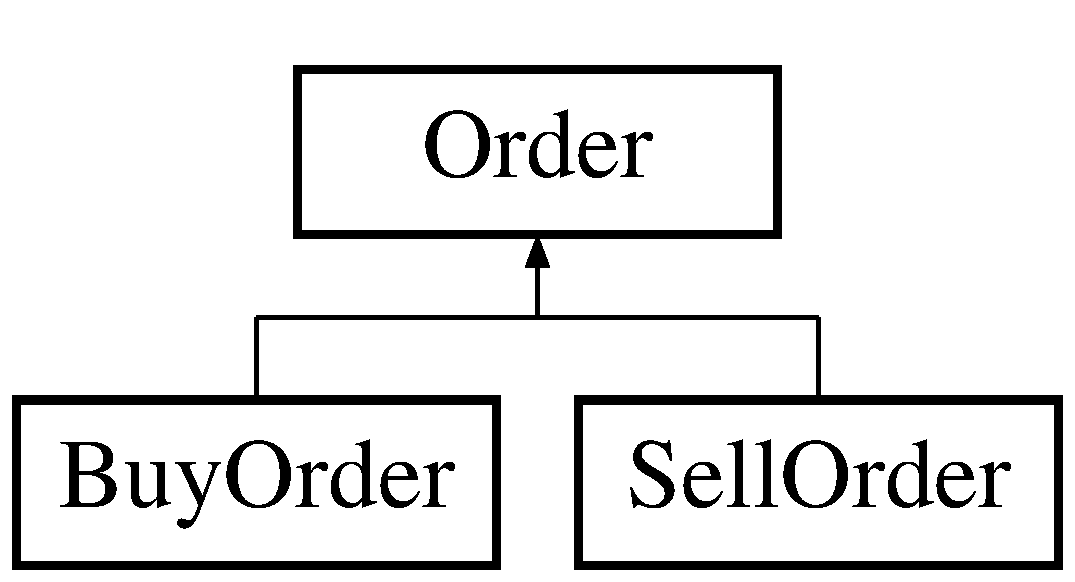
\includegraphics[height=2.000000cm]{class_order}
\end{center}
\end{figure}
\subsection*{Classes}
\begin{DoxyCompactItemize}
\item 
class \hyperlink{class_order_1_1_invalid_value}{Invalid\+Value}
\end{DoxyCompactItemize}
\subsection*{Public Member Functions}
\begin{DoxyCompactItemize}
\item 
\hyperlink{class_order_afd9bc0f1cf5ad376154ffde0e2727fbb}{Order} (ifstream \&in)
\item 
\hyperlink{class_order_afdda61d21957bffaf29e666ee6741bdc}{Order} (string s, double value, unsigned quant)
\item 
virtual \hyperlink{class_order_aa29be853510781d514722f857ab1698a}{$\sim$\+Order} ()=default
\item 
\hyperlink{class_date}{Date} \hyperlink{class_order_a8ffb9095f78f8a3b1942e7995516007c}{get\+Date\+Placed} () const
\item 
string \hyperlink{class_order_aa008956fd77ac3d254117443b7d916fa}{get\+Stock} () const
\item 
double \hyperlink{class_order_a7e93f84ff8b0468aef7e7ee23ea1979c}{get\+Value} () const
\item 
unsigned \hyperlink{class_order_a1d34436da1dbc3ffad588505eca5ff49}{get\+Quantity} () const
\item 
void \hyperlink{class_order_a718aea4e96286f2333222d6414eaa317}{print\+Info} () const
\item 
virtual nif\+\_\+t \hyperlink{class_order_a9831f386726f74ee20eea13a46282e13}{get\+Client\+N\+IF} () const =0
\item 
virtual \hyperlink{class_transaction}{Transaction} $\ast$ \hyperlink{class_order_a85d5de18c8664085619e3a5c74d47a25}{operator()} (\hyperlink{class_order}{Order} $\ast$o)=0
\item 
virtual void \hyperlink{class_order_a83989bde0a9b40cbeb0e87c965f6096e}{save\+Changes} (ofstream \&out) const
\end{DoxyCompactItemize}
\subsection*{Protected Attributes}
\begin{DoxyCompactItemize}
\item 
string \hyperlink{class_order_aafb6dfab2a1c253eefd78840b27dcd2e}{stock}
\item 
double \hyperlink{class_order_ab5d512fb35483413b9fe200d58324c2e}{value\+Per\+Stock}
\item 
unsigned \hyperlink{class_order_ab02e2baeb8c57217a20c9124df3ba11d}{quantity}
\item 
\hyperlink{class_date}{Date} \hyperlink{class_order_a23f58bb3f0162aac8c91a8a14136990c}{date\+Placed}
\end{DoxyCompactItemize}


\subsection{Detailed Description}
Abstract Base class used to represent an order. 

\subsection{Constructor \& Destructor Documentation}
\hypertarget{class_order_afd9bc0f1cf5ad376154ffde0e2727fbb}{}\label{class_order_afd9bc0f1cf5ad376154ffde0e2727fbb} 
\index{Order@{Order}!Order@{Order}}
\index{Order@{Order}!Order@{Order}}
\subsubsection{\texorpdfstring{Order()}{Order()}\hspace{0.1cm}{\footnotesize\ttfamily [1/2]}}
{\footnotesize\ttfamily Order\+::\+Order (\begin{DoxyParamCaption}\item[{ifstream \&}]{in }\end{DoxyParamCaption})}

A constructor. The construtor creates an order object, reading the data from the input stream passed as argument. 
\begin{DoxyParams}{Parameters}
{\em in} & The input stream to read from in order to build the order object. \\
\hline
\end{DoxyParams}
\hypertarget{class_order_afdda61d21957bffaf29e666ee6741bdc}{}\label{class_order_afdda61d21957bffaf29e666ee6741bdc} 
\index{Order@{Order}!Order@{Order}}
\index{Order@{Order}!Order@{Order}}
\subsubsection{\texorpdfstring{Order()}{Order()}\hspace{0.1cm}{\footnotesize\ttfamily [2/2]}}
{\footnotesize\ttfamily Order\+::\+Order (\begin{DoxyParamCaption}\item[{string}]{s,  }\item[{double}]{value,  }\item[{unsigned}]{quant }\end{DoxyParamCaption})}

A constructor. The construtor creates an order object using the data passed as arguments. 
\begin{DoxyParams}{Parameters}
{\em s} & A string with the stock name. \\
\hline
{\em value} & A double with the value per stock. \\
\hline
{\em quant} & An unsigned with the stock quantity. \\
\hline
\end{DoxyParams}
\hypertarget{class_order_aa29be853510781d514722f857ab1698a}{}\label{class_order_aa29be853510781d514722f857ab1698a} 
\index{Order@{Order}!````~Order@{$\sim$\+Order}}
\index{````~Order@{$\sim$\+Order}!Order@{Order}}
\subsubsection{\texorpdfstring{$\sim$\+Order()}{~Order()}}
{\footnotesize\ttfamily virtual Order\+::$\sim$\+Order (\begin{DoxyParamCaption}{ }\end{DoxyParamCaption})\hspace{0.3cm}{\ttfamily [virtual]}, {\ttfamily [default]}}

A virtual destructor. 

\subsection{Member Function Documentation}
\hypertarget{class_order_a9831f386726f74ee20eea13a46282e13}{}\label{class_order_a9831f386726f74ee20eea13a46282e13} 
\index{Order@{Order}!get\+Client\+N\+IF@{get\+Client\+N\+IF}}
\index{get\+Client\+N\+IF@{get\+Client\+N\+IF}!Order@{Order}}
\subsubsection{\texorpdfstring{get\+Client\+N\+I\+F()}{getClientNIF()}}
{\footnotesize\ttfamily virtual nif\+\_\+t Order\+::get\+Client\+N\+IF (\begin{DoxyParamCaption}{ }\end{DoxyParamCaption}) const\hspace{0.3cm}{\ttfamily [pure virtual]}}

A const abstract member function that returns the N\+IF of the client associated with the \hyperlink{class_order}{Order}. \begin{DoxyReturn}{Returns}
The N\+IF of the Buyer/\+Seller associated with the \hyperlink{class_order}{Order}. 
\end{DoxyReturn}


Implemented in \hyperlink{class_sell_order_a2f34e30d8bc5c891c40d8b80342cc34d}{Sell\+Order}, and \hyperlink{class_buy_order_ab79597b9bf0656216b2283bfa3a650e0}{Buy\+Order}.

\hypertarget{class_order_a8ffb9095f78f8a3b1942e7995516007c}{}\label{class_order_a8ffb9095f78f8a3b1942e7995516007c} 
\index{Order@{Order}!get\+Date\+Placed@{get\+Date\+Placed}}
\index{get\+Date\+Placed@{get\+Date\+Placed}!Order@{Order}}
\subsubsection{\texorpdfstring{get\+Date\+Placed()}{getDatePlaced()}}
{\footnotesize\ttfamily \hyperlink{class_date}{Date} Order\+::get\+Date\+Placed (\begin{DoxyParamCaption}{ }\end{DoxyParamCaption}) const}

A const member function with no arguments to get the orders\textquotesingle{}s place date. \begin{DoxyReturn}{Returns}
A \hyperlink{class_date}{Date} object , the date when the order was placed. 
\end{DoxyReturn}
\hypertarget{class_order_a1d34436da1dbc3ffad588505eca5ff49}{}\label{class_order_a1d34436da1dbc3ffad588505eca5ff49} 
\index{Order@{Order}!get\+Quantity@{get\+Quantity}}
\index{get\+Quantity@{get\+Quantity}!Order@{Order}}
\subsubsection{\texorpdfstring{get\+Quantity()}{getQuantity()}}
{\footnotesize\ttfamily unsigned Order\+::get\+Quantity (\begin{DoxyParamCaption}{ }\end{DoxyParamCaption}) const}

A const member function with no arguments to get the order stock quantity. \begin{DoxyReturn}{Returns}
An unsigned, the quantity of stock. 
\end{DoxyReturn}
\hypertarget{class_order_aa008956fd77ac3d254117443b7d916fa}{}\label{class_order_aa008956fd77ac3d254117443b7d916fa} 
\index{Order@{Order}!get\+Stock@{get\+Stock}}
\index{get\+Stock@{get\+Stock}!Order@{Order}}
\subsubsection{\texorpdfstring{get\+Stock()}{getStock()}}
{\footnotesize\ttfamily string Order\+::get\+Stock (\begin{DoxyParamCaption}{ }\end{DoxyParamCaption}) const}

A const member function with no arguments to get the orders\textquotesingle{}s stock name. \begin{DoxyReturn}{Returns}
A string that is the name of the stock. 
\end{DoxyReturn}
\hypertarget{class_order_a7e93f84ff8b0468aef7e7ee23ea1979c}{}\label{class_order_a7e93f84ff8b0468aef7e7ee23ea1979c} 
\index{Order@{Order}!get\+Value@{get\+Value}}
\index{get\+Value@{get\+Value}!Order@{Order}}
\subsubsection{\texorpdfstring{get\+Value()}{getValue()}}
{\footnotesize\ttfamily double Order\+::get\+Value (\begin{DoxyParamCaption}{ }\end{DoxyParamCaption}) const}

A const member function with no arguments to get the value per stock. \begin{DoxyReturn}{Returns}
A double, the value per stock. 
\end{DoxyReturn}
\hypertarget{class_order_a85d5de18c8664085619e3a5c74d47a25}{}\label{class_order_a85d5de18c8664085619e3a5c74d47a25} 
\index{Order@{Order}!operator()@{operator()}}
\index{operator()@{operator()}!Order@{Order}}
\subsubsection{\texorpdfstring{operator()()}{operator()()}}
{\footnotesize\ttfamily virtual \hyperlink{class_transaction}{Transaction}$\ast$ Order\+::operator() (\begin{DoxyParamCaption}\item[{\hyperlink{class_order}{Order} $\ast$}]{o }\end{DoxyParamCaption})\hspace{0.3cm}{\ttfamily [pure virtual]}}

Abstract overload of function operator. Cheks whether this instance of an \hyperlink{class_order}{Order} Object can be fulfilled by the provided \hyperlink{class_order}{Order}. 
\begin{DoxyParams}{Parameters}
{\em an} & \hyperlink{class_order}{Order} pointer \\
\hline
\end{DoxyParams}
\begin{DoxyReturn}{Returns}
A pointer to the transaction generated if successful, N\+U\+LL otherwise. 
\end{DoxyReturn}


Implemented in \hyperlink{class_sell_order_ae4e19807431bcd87c7126d0c644ff209}{Sell\+Order}, and \hyperlink{class_buy_order_a45641eed13ea191fff675745a618b9f5}{Buy\+Order}.

\hypertarget{class_order_a718aea4e96286f2333222d6414eaa317}{}\label{class_order_a718aea4e96286f2333222d6414eaa317} 
\index{Order@{Order}!print\+Info@{print\+Info}}
\index{print\+Info@{print\+Info}!Order@{Order}}
\subsubsection{\texorpdfstring{print\+Info()}{printInfo()}}
{\footnotesize\ttfamily void Order\+::print\+Info (\begin{DoxyParamCaption}{ }\end{DoxyParamCaption}) const}

A const member function that prints the order\textquotesingle{}s information to the standard output stream (cout). \hypertarget{class_order_a83989bde0a9b40cbeb0e87c965f6096e}{}\label{class_order_a83989bde0a9b40cbeb0e87c965f6096e} 
\index{Order@{Order}!save\+Changes@{save\+Changes}}
\index{save\+Changes@{save\+Changes}!Order@{Order}}
\subsubsection{\texorpdfstring{save\+Changes()}{saveChanges()}}
{\footnotesize\ttfamily void Order\+::save\+Changes (\begin{DoxyParamCaption}\item[{ofstream \&}]{out }\end{DoxyParamCaption}) const\hspace{0.3cm}{\ttfamily [virtual]}}

A virtual function to save changes in the derived classes. 

Reimplemented in \hyperlink{class_sell_order_a81c6ea39652c38a718803c036767787f}{Sell\+Order}, and \hyperlink{class_buy_order_aa4f087d0dbc1f6e8937c0b3679fc2f7b}{Buy\+Order}.



\subsection{Member Data Documentation}
\hypertarget{class_order_a23f58bb3f0162aac8c91a8a14136990c}{}\label{class_order_a23f58bb3f0162aac8c91a8a14136990c} 
\index{Order@{Order}!date\+Placed@{date\+Placed}}
\index{date\+Placed@{date\+Placed}!Order@{Order}}
\subsubsection{\texorpdfstring{date\+Placed}{datePlaced}}
{\footnotesize\ttfamily \hyperlink{class_date}{Date} Order\+::date\+Placed\hspace{0.3cm}{\ttfamily [protected]}}

\hyperlink{class_date}{Date} date\+Placed. The date when the order was placed. \hypertarget{class_order_ab02e2baeb8c57217a20c9124df3ba11d}{}\label{class_order_ab02e2baeb8c57217a20c9124df3ba11d} 
\index{Order@{Order}!quantity@{quantity}}
\index{quantity@{quantity}!Order@{Order}}
\subsubsection{\texorpdfstring{quantity}{quantity}}
{\footnotesize\ttfamily unsigned Order\+::quantity\hspace{0.3cm}{\ttfamily [protected]}}

unsigned quantity. An unsigned with the stock quantity. \hypertarget{class_order_aafb6dfab2a1c253eefd78840b27dcd2e}{}\label{class_order_aafb6dfab2a1c253eefd78840b27dcd2e} 
\index{Order@{Order}!stock@{stock}}
\index{stock@{stock}!Order@{Order}}
\subsubsection{\texorpdfstring{stock}{stock}}
{\footnotesize\ttfamily string Order\+::stock\hspace{0.3cm}{\ttfamily [protected]}}

string stock. A string with stock name. \hypertarget{class_order_ab5d512fb35483413b9fe200d58324c2e}{}\label{class_order_ab5d512fb35483413b9fe200d58324c2e} 
\index{Order@{Order}!value\+Per\+Stock@{value\+Per\+Stock}}
\index{value\+Per\+Stock@{value\+Per\+Stock}!Order@{Order}}
\subsubsection{\texorpdfstring{value\+Per\+Stock}{valuePerStock}}
{\footnotesize\ttfamily double Order\+::value\+Per\+Stock\hspace{0.3cm}{\ttfamily [protected]}}

value\+Per\+Stock. A double with the stock value. 

The documentation for this class was generated from the following files\+:\begin{DoxyCompactItemize}
\item 
Order.\+h\item 
Order.\+cpp\end{DoxyCompactItemize}

\hypertarget{class_sell_order}{}\section{Sell\+Order Class Reference}
\label{class_sell_order}\index{Sell\+Order@{Sell\+Order}}


{\ttfamily \#include $<$Order.\+h$>$}

Inheritance diagram for Sell\+Order\+:\begin{figure}[H]
\begin{center}
\leavevmode
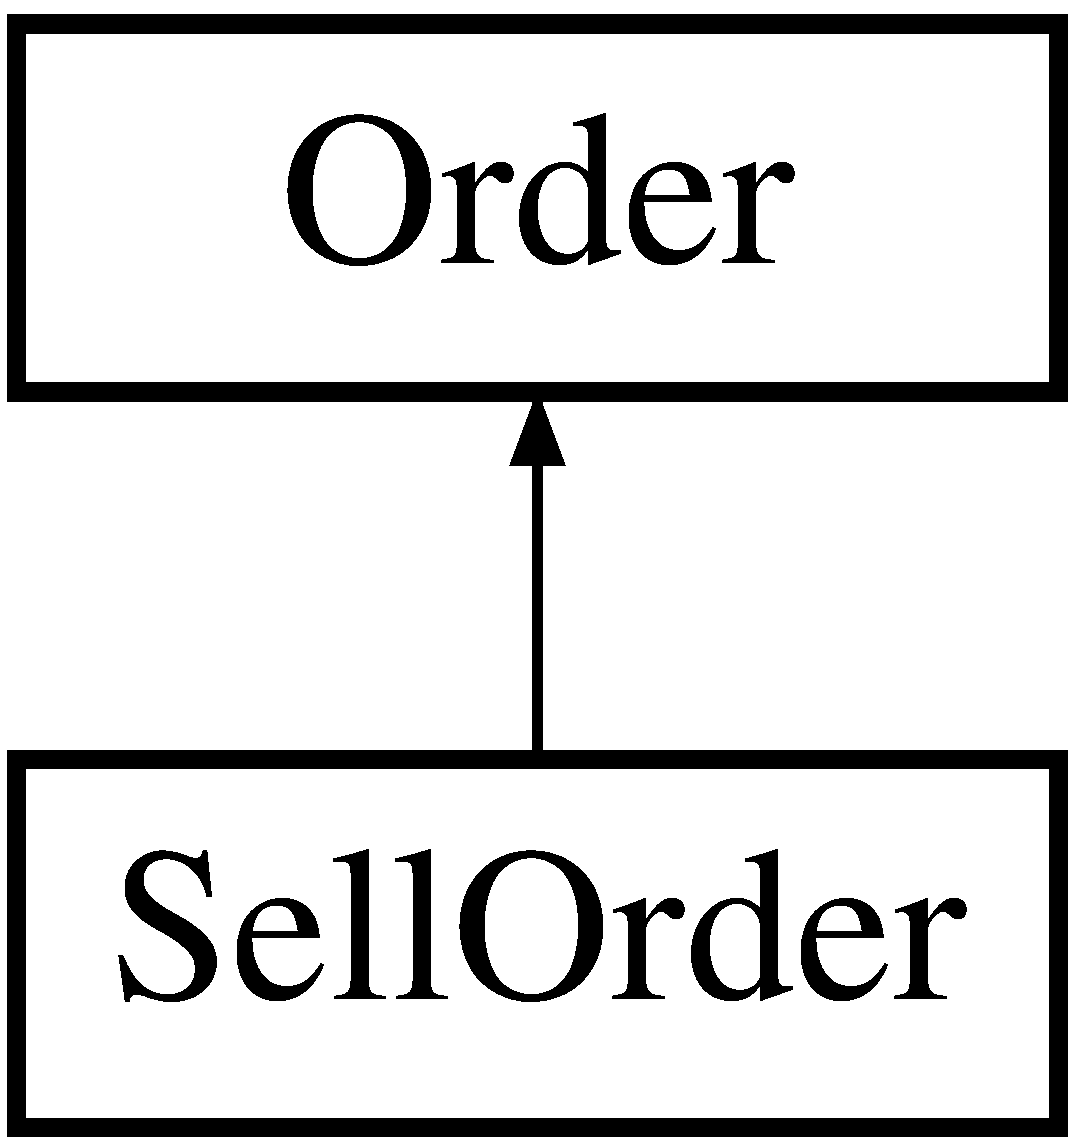
\includegraphics[height=2.000000cm]{class_sell_order}
\end{center}
\end{figure}
\subsection*{Public Member Functions}
\begin{DoxyCompactItemize}
\item 
\hyperlink{class_sell_order_ac89fdde112f2f9aac52633a2d9507bea}{Sell\+Order} (ifstream \&in)
\begin{DoxyCompactList}\small\item\em /// \end{DoxyCompactList}\item 
\hyperlink{class_sell_order_a19145616a9cceec182bdcb00816b89c5}{Sell\+Order} (string \hyperlink{class_order_aafb6dfab2a1c253eefd78840b27dcd2e}{stock}, double val, unsigned \hyperlink{class_order_ab02e2baeb8c57217a20c9124df3ba11d}{quantity}, nif\+\_\+t seller\+N\+IF)
\item 
nif\+\_\+t \hyperlink{class_sell_order_a2f34e30d8bc5c891c40d8b80342cc34d}{get\+Client\+N\+IF} () const
\item 
\hyperlink{class_transaction}{Transaction} $\ast$ \hyperlink{class_sell_order_ae4e19807431bcd87c7126d0c644ff209}{operator()} (\hyperlink{class_order}{Order} $\ast$o)
\item 
void \hyperlink{class_sell_order_a81c6ea39652c38a718803c036767787f}{save\+Changes} (ofstream \&out) const
\end{DoxyCompactItemize}
\subsection*{Additional Inherited Members}


\subsection{Detailed Description}
Class used to represent a sell order. Derives from \hyperlink{class_order}{Order}. 

\subsection{Constructor \& Destructor Documentation}
\hypertarget{class_sell_order_ac89fdde112f2f9aac52633a2d9507bea}{}\label{class_sell_order_ac89fdde112f2f9aac52633a2d9507bea} 
\index{Sell\+Order@{Sell\+Order}!Sell\+Order@{Sell\+Order}}
\index{Sell\+Order@{Sell\+Order}!Sell\+Order@{Sell\+Order}}
\subsubsection{\texorpdfstring{Sell\+Order()}{SellOrder()}\hspace{0.1cm}{\footnotesize\ttfamily [1/2]}}
{\footnotesize\ttfamily Sell\+Order\+::\+Sell\+Order (\begin{DoxyParamCaption}\item[{ifstream \&}]{in }\end{DoxyParamCaption})}



/// 

A constructor. The construtor creates a \hyperlink{class_sell_order}{Sell\+Order} object, reading the data from the input stream passed as argument. 
\begin{DoxyParams}{Parameters}
{\em in} & The input stream to read from in order to build the \hyperlink{class_sell_order}{Sell\+Order} object. \\
\hline
\end{DoxyParams}
\hypertarget{class_sell_order_a19145616a9cceec182bdcb00816b89c5}{}\label{class_sell_order_a19145616a9cceec182bdcb00816b89c5} 
\index{Sell\+Order@{Sell\+Order}!Sell\+Order@{Sell\+Order}}
\index{Sell\+Order@{Sell\+Order}!Sell\+Order@{Sell\+Order}}
\subsubsection{\texorpdfstring{Sell\+Order()}{SellOrder()}\hspace{0.1cm}{\footnotesize\ttfamily [2/2]}}
{\footnotesize\ttfamily Sell\+Order\+::\+Sell\+Order (\begin{DoxyParamCaption}\item[{string}]{stock,  }\item[{double}]{val,  }\item[{unsigned}]{quantity,  }\item[{nif\+\_\+t}]{seller\+N\+IF }\end{DoxyParamCaption})}

A constructor. The construtor creates a \hyperlink{class_sell_order}{Sell\+Order} object using the data passed as arguments. 
\begin{DoxyParams}{Parameters}
{\em stock} & A string with the stock name. \\
\hline
{\em val} & A double with the value per stock. \\
\hline
{\em quantity} & An unsigned with the stock quantity. \\
\hline
{\em seller\+N\+IF} & The seller\textquotesingle{}s N\+IF. \\
\hline
\end{DoxyParams}


\subsection{Member Function Documentation}
\hypertarget{class_sell_order_a2f34e30d8bc5c891c40d8b80342cc34d}{}\label{class_sell_order_a2f34e30d8bc5c891c40d8b80342cc34d} 
\index{Sell\+Order@{Sell\+Order}!get\+Client\+N\+IF@{get\+Client\+N\+IF}}
\index{get\+Client\+N\+IF@{get\+Client\+N\+IF}!Sell\+Order@{Sell\+Order}}
\subsubsection{\texorpdfstring{get\+Client\+N\+I\+F()}{getClientNIF()}}
{\footnotesize\ttfamily nif\+\_\+t Sell\+Order\+::get\+Client\+N\+IF (\begin{DoxyParamCaption}{ }\end{DoxyParamCaption}) const\hspace{0.3cm}{\ttfamily [virtual]}}

A const member function that returns the N\+IF of the client associated with this \hyperlink{class_sell_order}{Sell\+Order}. \begin{DoxyReturn}{Returns}
The N\+IF of the Seller associated with this \hyperlink{class_order}{Order}. 
\end{DoxyReturn}


Implements \hyperlink{class_order_a9831f386726f74ee20eea13a46282e13}{Order}.

\hypertarget{class_sell_order_ae4e19807431bcd87c7126d0c644ff209}{}\label{class_sell_order_ae4e19807431bcd87c7126d0c644ff209} 
\index{Sell\+Order@{Sell\+Order}!operator()@{operator()}}
\index{operator()@{operator()}!Sell\+Order@{Sell\+Order}}
\subsubsection{\texorpdfstring{operator()()}{operator()()}}
{\footnotesize\ttfamily \hyperlink{class_transaction}{Transaction} $\ast$ Sell\+Order\+::operator() (\begin{DoxyParamCaption}\item[{\hyperlink{class_order}{Order} $\ast$}]{o }\end{DoxyParamCaption})\hspace{0.3cm}{\ttfamily [virtual]}}

Overload of operator() for class \hyperlink{class_order}{Order}. 
\begin{DoxyParams}{Parameters}
{\em o} & Pointer of an object \hyperlink{class_order}{Order}. \\
\hline
\end{DoxyParams}
\begin{DoxyReturn}{Returns}
A transaction type object. 
\end{DoxyReturn}


Implements \hyperlink{class_order_a85d5de18c8664085619e3a5c74d47a25}{Order}.

\hypertarget{class_sell_order_a81c6ea39652c38a718803c036767787f}{}\label{class_sell_order_a81c6ea39652c38a718803c036767787f} 
\index{Sell\+Order@{Sell\+Order}!save\+Changes@{save\+Changes}}
\index{save\+Changes@{save\+Changes}!Sell\+Order@{Sell\+Order}}
\subsubsection{\texorpdfstring{save\+Changes()}{saveChanges()}}
{\footnotesize\ttfamily void Sell\+Order\+::save\+Changes (\begin{DoxyParamCaption}\item[{ofstream \&}]{out }\end{DoxyParamCaption}) const\hspace{0.3cm}{\ttfamily [virtual]}}

A const memeber function to save changes in an output stream. 
\begin{DoxyParams}{Parameters}
{\em out} & The outstream file to write to. \\
\hline
\end{DoxyParams}


Reimplemented from \hyperlink{class_order_a83989bde0a9b40cbeb0e87c965f6096e}{Order}.



The documentation for this class was generated from the following files\+:\begin{DoxyCompactItemize}
\item 
Order.\+h\item 
Order.\+cpp\end{DoxyCompactItemize}

\hypertarget{class_transaction}{}\section{Transaction Class Reference}
\label{class_transaction}\index{Transaction@{Transaction}}


{\ttfamily \#include $<$Transaction.\+h$>$}

\subsection*{Public Member Functions}
\begin{DoxyCompactItemize}
\item 
\hyperlink{class_transaction_a0c8031bed6e7a45eda7bc2ca8f40e851}{Transaction} ()=default
\item 
\hyperlink{class_transaction_a2bbb78694a94a630cb1e9e741dc120a7}{Transaction} (ifstream \&in)
\item 
\hyperlink{class_transaction_abd1826b5a0499ddac290a4f1297e7455}{Transaction} (nif\+\_\+t buyer\+N\+IF, nif\+\_\+t seller\+N\+IF, string stock, double value, unsigned quantity)
\item 
string \hyperlink{class_transaction_af6582ddc59e9cfa99a7ef178216799be}{get\+Stock} () const
\item 
double \hyperlink{class_transaction_a95976b2e60b66d766edf4db534324db4}{get\+Value} () const
\item 
unsigned \hyperlink{class_transaction_ab3bfaa0469e1f45c5bd5dc164ac3c850}{get\+Quantity} () const
\item 
nif\+\_\+t \hyperlink{class_transaction_a3c3a57a3240bece392c56ff41bc3c21b}{get\+Seller\+N\+IF} () const
\item 
nif\+\_\+t \hyperlink{class_transaction_afa91c88bb936d8bd8480ac36b599649b}{get\+Buyer\+N\+IF} () const
\item 
\hyperlink{class_date}{Date} \hyperlink{class_transaction_af2ef4a1ef82f9ff5d34dae7234211589}{get\+Date} () const
\item 
void \hyperlink{class_transaction_a3c0c3c4a64c5b3d20c420708357a86be}{save\+Changes} (ofstream \&out) const
\end{DoxyCompactItemize}
\subsection*{Friends}
\begin{DoxyCompactItemize}
\item 
ostream \& \hyperlink{class_transaction_a75af23fbc3b593013d411cf50c5a3a7a}{operator$<$$<$} (ostream \&out, const \hyperlink{class_transaction}{Transaction} \&t)
\end{DoxyCompactItemize}


\subsection{Detailed Description}
A class used to represent a transaction. 

\subsection{Constructor \& Destructor Documentation}
\hypertarget{class_transaction_a0c8031bed6e7a45eda7bc2ca8f40e851}{}\label{class_transaction_a0c8031bed6e7a45eda7bc2ca8f40e851} 
\index{Transaction@{Transaction}!Transaction@{Transaction}}
\index{Transaction@{Transaction}!Transaction@{Transaction}}
\subsubsection{\texorpdfstring{Transaction()}{Transaction()}\hspace{0.1cm}{\footnotesize\ttfamily [1/3]}}
{\footnotesize\ttfamily Transaction\+::\+Transaction (\begin{DoxyParamCaption}{ }\end{DoxyParamCaption})\hspace{0.3cm}{\ttfamily [default]}}

A default constructor. \hypertarget{class_transaction_a2bbb78694a94a630cb1e9e741dc120a7}{}\label{class_transaction_a2bbb78694a94a630cb1e9e741dc120a7} 
\index{Transaction@{Transaction}!Transaction@{Transaction}}
\index{Transaction@{Transaction}!Transaction@{Transaction}}
\subsubsection{\texorpdfstring{Transaction()}{Transaction()}\hspace{0.1cm}{\footnotesize\ttfamily [2/3]}}
{\footnotesize\ttfamily Transaction\+::\+Transaction (\begin{DoxyParamCaption}\item[{ifstream \&}]{in }\end{DoxyParamCaption})}

A constructor. The construtor creates a transaction object, reading the data from the input stream passed as argument. 
\begin{DoxyParams}{Parameters}
{\em in} & The input stream to read from in order to build the transaction object. \\
\hline
\end{DoxyParams}
\hypertarget{class_transaction_abd1826b5a0499ddac290a4f1297e7455}{}\label{class_transaction_abd1826b5a0499ddac290a4f1297e7455} 
\index{Transaction@{Transaction}!Transaction@{Transaction}}
\index{Transaction@{Transaction}!Transaction@{Transaction}}
\subsubsection{\texorpdfstring{Transaction()}{Transaction()}\hspace{0.1cm}{\footnotesize\ttfamily [3/3]}}
{\footnotesize\ttfamily Transaction\+::\+Transaction (\begin{DoxyParamCaption}\item[{nif\+\_\+t}]{buyer\+N\+IF,  }\item[{nif\+\_\+t}]{seller\+N\+IF,  }\item[{string}]{stock,  }\item[{double}]{value,  }\item[{unsigned}]{quantity }\end{DoxyParamCaption})}

A constructor. The construtor creates a transaction object using the data passed as arguments. 
\begin{DoxyParams}{Parameters}
{\em buyer\+N\+IF} & The N\+IF from the buyer. \\
\hline
{\em seller\+N\+IF} & The N\+IF from the seller. \\
\hline
{\em stock} & The stock name. \\
\hline
{\em value} & The value of the stock. \\
\hline
{\em quantity} & The amount of stock. \\
\hline
\end{DoxyParams}


\subsection{Member Function Documentation}
\hypertarget{class_transaction_afa91c88bb936d8bd8480ac36b599649b}{}\label{class_transaction_afa91c88bb936d8bd8480ac36b599649b} 
\index{Transaction@{Transaction}!get\+Buyer\+N\+IF@{get\+Buyer\+N\+IF}}
\index{get\+Buyer\+N\+IF@{get\+Buyer\+N\+IF}!Transaction@{Transaction}}
\subsubsection{\texorpdfstring{get\+Buyer\+N\+I\+F()}{getBuyerNIF()}}
{\footnotesize\ttfamily nif\+\_\+t Transaction\+::get\+Buyer\+N\+IF (\begin{DoxyParamCaption}{ }\end{DoxyParamCaption}) const}

A const member function with no arguments to get the transaction\textquotesingle{}s buyer N\+IF. \begin{DoxyReturn}{Returns}
A nif\+\_\+t , the buyer N\+IF. 
\end{DoxyReturn}
\hypertarget{class_transaction_af2ef4a1ef82f9ff5d34dae7234211589}{}\label{class_transaction_af2ef4a1ef82f9ff5d34dae7234211589} 
\index{Transaction@{Transaction}!get\+Date@{get\+Date}}
\index{get\+Date@{get\+Date}!Transaction@{Transaction}}
\subsubsection{\texorpdfstring{get\+Date()}{getDate()}}
{\footnotesize\ttfamily \hyperlink{class_date}{Date} Transaction\+::get\+Date (\begin{DoxyParamCaption}{ }\end{DoxyParamCaption}) const}

A const member function with no arguments to get the transaction\textquotesingle{}s date. \begin{DoxyReturn}{Returns}
A \hyperlink{class_date}{Date} object , the date of the transaction. 
\end{DoxyReturn}
\hypertarget{class_transaction_ab3bfaa0469e1f45c5bd5dc164ac3c850}{}\label{class_transaction_ab3bfaa0469e1f45c5bd5dc164ac3c850} 
\index{Transaction@{Transaction}!get\+Quantity@{get\+Quantity}}
\index{get\+Quantity@{get\+Quantity}!Transaction@{Transaction}}
\subsubsection{\texorpdfstring{get\+Quantity()}{getQuantity()}}
{\footnotesize\ttfamily unsigned Transaction\+::get\+Quantity (\begin{DoxyParamCaption}{ }\end{DoxyParamCaption}) const}

A const member function with no arguments to get the transaction\textquotesingle{}s quantity of stock. \begin{DoxyReturn}{Returns}
An unsigned, the quantity. 
\end{DoxyReturn}
\hypertarget{class_transaction_a3c3a57a3240bece392c56ff41bc3c21b}{}\label{class_transaction_a3c3a57a3240bece392c56ff41bc3c21b} 
\index{Transaction@{Transaction}!get\+Seller\+N\+IF@{get\+Seller\+N\+IF}}
\index{get\+Seller\+N\+IF@{get\+Seller\+N\+IF}!Transaction@{Transaction}}
\subsubsection{\texorpdfstring{get\+Seller\+N\+I\+F()}{getSellerNIF()}}
{\footnotesize\ttfamily nif\+\_\+t Transaction\+::get\+Seller\+N\+IF (\begin{DoxyParamCaption}{ }\end{DoxyParamCaption}) const}

A const member function with no arguments to get the transaction\textquotesingle{}s seller N\+IF. \begin{DoxyReturn}{Returns}
A nif\+\_\+t , the seller N\+IF. 
\end{DoxyReturn}
\hypertarget{class_transaction_af6582ddc59e9cfa99a7ef178216799be}{}\label{class_transaction_af6582ddc59e9cfa99a7ef178216799be} 
\index{Transaction@{Transaction}!get\+Stock@{get\+Stock}}
\index{get\+Stock@{get\+Stock}!Transaction@{Transaction}}
\subsubsection{\texorpdfstring{get\+Stock()}{getStock()}}
{\footnotesize\ttfamily string Transaction\+::get\+Stock (\begin{DoxyParamCaption}{ }\end{DoxyParamCaption}) const}

A const member function with no arguments to get the transaction\textquotesingle{}s Stock name. \begin{DoxyReturn}{Returns}
A string, the Stock\textquotesingle{}s name. 
\end{DoxyReturn}
\hypertarget{class_transaction_a95976b2e60b66d766edf4db534324db4}{}\label{class_transaction_a95976b2e60b66d766edf4db534324db4} 
\index{Transaction@{Transaction}!get\+Value@{get\+Value}}
\index{get\+Value@{get\+Value}!Transaction@{Transaction}}
\subsubsection{\texorpdfstring{get\+Value()}{getValue()}}
{\footnotesize\ttfamily double Transaction\+::get\+Value (\begin{DoxyParamCaption}{ }\end{DoxyParamCaption}) const}

A const member function with no arguments to get the transaction\textquotesingle{}s Value Per Stock. \begin{DoxyReturn}{Returns}
A double, the value per stock transactioned. 
\end{DoxyReturn}
\hypertarget{class_transaction_a3c0c3c4a64c5b3d20c420708357a86be}{}\label{class_transaction_a3c0c3c4a64c5b3d20c420708357a86be} 
\index{Transaction@{Transaction}!save\+Changes@{save\+Changes}}
\index{save\+Changes@{save\+Changes}!Transaction@{Transaction}}
\subsubsection{\texorpdfstring{save\+Changes()}{saveChanges()}}
{\footnotesize\ttfamily void Transaction\+::save\+Changes (\begin{DoxyParamCaption}\item[{ofstream \&}]{out }\end{DoxyParamCaption}) const}

A const member function to write the transaction to a save file. 
\begin{DoxyParams}{Parameters}
{\em out} & The outputstream file to write to. \\
\hline
\end{DoxyParams}


\subsection{Friends And Related Function Documentation}
\hypertarget{class_transaction_a75af23fbc3b593013d411cf50c5a3a7a}{}\label{class_transaction_a75af23fbc3b593013d411cf50c5a3a7a} 
\index{Transaction@{Transaction}!operator$<$$<$@{operator$<$$<$}}
\index{operator$<$$<$@{operator$<$$<$}!Transaction@{Transaction}}
\subsubsection{\texorpdfstring{operator$<$$<$}{operator<<}}
{\footnotesize\ttfamily ostream\& operator$<$$<$ (\begin{DoxyParamCaption}\item[{ostream \&}]{out,  }\item[{const \hyperlink{class_transaction}{Transaction} \&}]{t }\end{DoxyParamCaption})\hspace{0.3cm}{\ttfamily [friend]}}

Overload of Operator $<$$<$ for class \hyperlink{class_transaction}{Transaction}. Prints the transaction in a human friendly way. 
\begin{DoxyParams}{Parameters}
{\em out} & The outstream to write to. \\
\hline
{\em t} & The transaction to be written. \\
\hline
\end{DoxyParams}
\begin{DoxyReturn}{Returns}
Returns the output stream to allow chaining 
\end{DoxyReturn}


The documentation for this class was generated from the following files\+:\begin{DoxyCompactItemize}
\item 
Transaction.\+h\item 
Transaction.\+cpp\end{DoxyCompactItemize}

%--- End generated contents ---

% Index
\backmatter
\newpage
\phantomsection
\clearemptydoublepage
\addcontentsline{toc}{chapter}{Index}
\printindex

\end{document}
